\documentclass[twoside,11pt]{article}
\usepackage{jmlr2e}
\usepackage{amsmath}
\usepackage{algorithm}
\usepackage{algorithmicx}
\usepackage{algpseudocode}


\iffalse
\usepackage[utf8]{inputenc}
\usepackage{abstract}
\usepackage{geometry}
\geometry{a4paper,scale=0.75}
\usepackage{authblk}
\usepackage{algorithm}
\usepackage{algorithmicx}
\usepackage{algpseudocode}
\usepackage{amsmath}
\usepackage{graphicx}
\usepackage{chngcntr}
\counterwithout{figure}{section}
\usepackage{float}
\usepackage{titlesec}
\usepackage{titlepic}
\DeclareMathOperator*{\argmax}{argmax}
\usepackage[round]{natbib}
\bibliographystyle{plainnat}
\usepackage{amssymb}
\usepackage{amsthm}
\usepackage{hyperref}
\usepackage{tabularx,ragged2e}
\usepackage{nccmath}
\usepackage{caption}
\usepackage{flexisym}
\newcolumntype{C}{>{\Centering\arraybackslash}X}
\hypersetup{
    colorlinks=true,
    linkcolor=blue,
    filecolor=magenta,      
    citecolor=blue,
}
\newtheorem{theorem}{Theorem}
\newtheorem{definition}{Definition}[subsection]
\newtheorem{lemma}{Lemma}[subsection]
%\newtheorem{prop}{Proposition}[subsection]

\usepackage{caption}
\captionsetup[table]{position=bottom}
\usepackage[export]{adjustbox}

\usepackage{scalerel,stackengine}
\stackMath


\newcommand\widehat[1]{%
\savestack{\tmpbox}{\stretchto{%
  \scaleto{%
    \scalerel*[\widthof{\ensuremath{#1}}]{\kern-.6pt\bigwedge\kern-.6pt}%
    {\rule[-\textheight/2]{1ex}{\textheight}}%WIDTH-LIMITED BIG WEDGE
  }{\textheight}}% 
}{0.5ex}%
\stackon[1pt]{#1}{\tmpbox}%
}
\fi
\parskip 1ex


\newcommand{\dataset}{{\cal D}}
\newcommand{\fracpartial}[2]{\frac{\partial #1}{\partial  #2}}


%\jmlrheading{1}{2000}{1-48}{4/00}{10/00}{Marina Meil\u{a} and Michael I. Jordan}



%\ShortHeadings{Comonotone-Independence Bayesian Classifier}{Meil\u{a} and Jordan}
\firstpageno{1}

\begin{document}

\title{Comonotone-Independence Bayesian Classifier}
\author{}
\editor{}

% \author{\name Marina Meil\u{a} \email mmp@stat.washington.edu \\
%        \addr Department of Statistics\\
%        University of Washington\\
%        Seattle, WA 98195-4322, USA
%        \AND
%        \name Michael I.\ Jordan \email jordan@cs.berkeley.edu \\
%        \addr Division of Computer Science and Department of Statistics\\
%        University of California\\
%        Berkeley, CA 94720-1776, USA}

% \editor{Leslie Pack Kaelbling}

\maketitle

\begin{abstract}
    In the machine learning community, Na\"ive Bayes has been widely used not only as a classification model but also as a benchmark when evaluating new models. Due to its competitive performance and high efficiency in many scenarios, models aiming to refine it pursues a better performance while maintains a low complexity. In this paper, we propose a novel Bayesian classifier named Comonotone-Independence Bayesian Classifier (CIBer), which searches for an optimal partition of the predictive features, and then measure the conditional joint probability within each group of features by assuming they have comonotonic dependence structure. We shall not only explain and verify the conditions in which CIBer is globally optimal by a simulation study, but also confirm its competitiveness by applying it to several real-world domains. Since the ideology of CIBer is much different from previous refinements to Na\"ive Bayes, we directly compare CIBer's performance on real data-sets with classical methods including Na\"ive Bayes, Decision Tree, Support Vector Machine, Logistic Regression, and two state-of-the-art methods including Random Forest and XGBoost. Our experimental results demonstrate CIBer's competitiveness in classification tasks.
\end{abstract}

\begin{keywords}
  Bayesian Classifier, Comonotonicity, Conditional Independence, Heuristic Search, Hierarchical Clustering
\end{keywords}


\section{Introduction}
Na\"ive Bayes, the simplest but most efficient Bayesian classifier, has been widely used for many decades \citep{lewis1998naive, domingos1997optimality}. Given a vector containing multiple predictive features of an instance, a Bayesian classifier computes the probability for every possible label by the Bayes Theorem as shown in Definition \ref{def:1}.

\begin{definition}{Bayes theorem.}
\label{def:1}
 Suppose the input feature vector $\mathbf{X} = (X_1,\dots,X_d)$, and define the set of all labels as $\mathcal{C}$. Let $\mathbf{x}=(x_1,\dots,x_d)$ be a vector containing the observed value of predictive features, and let $y\in\mathcal{C}$ be a possible class, then
\begin{equation*}
    \mathbb{P}(y|\mathbf{x}) = \mathbb{P}(y)\cdot\frac{\mathbb{P}(\mathbf{x}|y)}{\mathbb{P}(\mathbf{x})}=\mathbb{P}(y)\cdot\frac{\mathbb{P}(\mathbf{x}|y)}{\sum_{y'\in\mathcal{C}}\mathbb{P}(\mathbf{x},y')}
\end{equation*}
\end{definition}

Thus, for an instance $\mathbf{x}$, a Bayesian classifier classifies it by computing the probability of it belonging to every possible label \citep{duda1973pattern}. Since the denominator $\sum_{y'\in\mathcal{C}}\mathbb{P}(\mathbf{x},y')$ is the same for each label, the class ultimately determined by a Bayesian classifier satisfies:
\begin{equation*}
    \label{eq:1}
    \centering
    y_{predict}=\mathop{\arg\max}\limits_{y} \mathbb{P}(\mathbf{x}|y)\cdot\mathbb{P}(y)
\end{equation*}

Since $\mathbb{P}(y)$ can be easily estimated by the proportion of the observations in class $y$ in the training set, the most crucial task for a Bayesian classifier is to estimate the conditional joint probability, i.e.,  $\mathbb{P}(\mathbf{x}|y)$. Theoretically, one can use the chain rule to calculate the joint probability by repeatedly applying the conditional probability. In the case of conditional joint probability, the calculation can be written as 
\begin{equation}
\begin{aligned}
    \mathbb{P}(\mathbf{x}|y) &= \mathbb{P}(x_1|x_2,\dots,x_d,y)\cdot\mathbb{P}(x_2,\dots,x_d|y) \\
    &=\mathbb{P}(x_1|x_2,\dots,x_d,y)\cdot\mathbb{P}(x_2|x_3,\dots,x_d,y)\cdot\mathbb{P}(x_3,\dots,x_d|y)\\
    &=\dots \\
    &=\mathbb{P}(x_1|x_2,\dots,x_d,y)\cdot\mathbb{P}(x_2|x_3,\dots,x_d,y)\dots\mathbb{P}(x_{d-1}|x_d,y)\cdot\mathbb{P}(x_d|y).\\
\end{aligned}
\label{actual_computation}
\end{equation}

However, computing the conditional joint probability by Equation \ref{actual_computation} is always impractical as it is very likely for $\mathbb{P}(x_i|x_{i+1},\dots,x_d,y)$ to be empirically immeasurable. In the discrete case, there might be no instance having $X_{i+1}=x_{i+1},\dots,X_d=x_d,Y=y$ for some small $i$'s, and thus results in the zero probability problem. When it comes to the continuous case, parametric models such as multivariate gaussian distribution are needed. However, such models make strong assumptions for the joint distribution in advance. In order to avoid these problems, Na\"ive Bayes makes an assumption that $X_1,\dots,X_d$ are conditionally independent, in which case we have Equation \ref{nb_equation}.
\begin{equation}
    \centering
    \mathbb{P}(\mathbf{x}|y)=\prod_{i=1}^{d}\mathbb{P}(x_i|y)
    \label{nb_equation}
\end{equation}

Since the set of samples having $X_i=x_i, Y=y$ must contain those having $X_i=x_i,X_{i+1}=x_{i+1},\dots,X_d=x_d,Y=y$, there are more samples to be counted in each conditional probability estimation, and thus effectively reduces the cases of zero probability. Meanwhile, the computation becomes more straightforward and reduces the complexity. Although in reality the conditional independence assumption is rarely satisfied, previous researches have verified its surprisingly strong competitiveness compared with more complex learning models, such as Decision Tree and Support Vector Machine \citep{dougherty1995supervised, huang2003comparing}. Moreover, \citet{zhang2004optimality} has investigated and proved the sufficient conditions for the optimality of Na\"ive Bayes. He demonstrated that no matter how strongly the features are dependent with each other, Na\"ive Bayes is optimal if either the dependence distribute evenly within each class or the dependence hedge each other properly.

However, in more common cases in which the optimal conditions do not hold, the violation of conditional independence makes the probability estimates suboptimal. Thus, there have been many literatures proposing improvements from different aspects to replace the na\"ive assumption. We make a review for these methods here.

In most cases, the na\"ive assumption of feature independence is violated, and result in a sub-optimal estimation of the conditional joint probability. Although there are literatures reasoning about the conditions for its optimality in classification \citep{domingos1996beyond,domingos1997optimality,zhang2004optimality}, a number of models trying to alleviate the inaccuracies caused by the assumption when such conditions for optimality do not hold have been proposed. These models can be roughly divided into three categories, namely, \textit{attribute weighting models}, \textit{semi-na\"ive Bayes models}, and \textit{Bayesian network}. In general, models in these three categories enhance the performance of Bayesian classifier from different aspects. In terms of attribute weighting, as claimed by \citet{zaidi2013alleviating}, even though it seems that assigning weights increases the impact from features with higher predictive power while reduces the impact from those with lower predictive power, the main value of attribute weighting is that it reduces the impact on the prediction accuracy when violating the conditional independence assumption, and thus improves the model performance. When it comes to semi-na\"ive Bayes models, the success is because it weakens the independence assumption by considering some dependencies among the features \citep{zheng2005comparative}. As for Bayesian network, it is more general than semi-na\"ive Bayes models since a more concrete graphical model, which is represented by a directed acyclic graph (DAG), is used to model causal or conditional independence relationships among the attributes. The previous works are reviewed separately by these categories.

\subsection{Attribute Weighting}
Models using the attribute weighting technique assign weights to each feature during the training process. If we assign a single weight $w_i$ to each $X_i$, then for any input $\mathbf{x}=(x_1,\dots,x_d)$ and any $y\in\mathcal{C}$, the probability $\mathbb{P}(y|\mathbf{x})$ is computed by.

\begin{equation*}
    \centering
    \mathbb{P}(y|\mathbf{x})=\frac{\mathbb{P}(y,\mathbf{x})}{\mathbb{P}(\mathbf{x})}=\frac{\mathbb{P}(y)\cdot\prod_{i=1}^{d}\mathbb{P}(x_i|y)^{w_i}}{\sum_{y'\in\mathcal{C}}\mathbb{P}(y')\cdot\prod_{i=1}^{d}\mathbb{P}(x_i|y')^{w_i}}.
\end{equation*}

The most crucial task becomes finding an optimal weight vector $\mathbf{w}=(w_1,\dots,w_d)$. Previous works related to attribute weighting can be roughly divided into two sub-categories, as shown below.

\begin{itemize}
    \item Using some mechanisms which increase the weights for features having larger predictive power while decrease the weights for those having smaller predictive power.
    \item Reducing the impact on the performance caused by violation of independence by iteratively optimizing the weight vector.
\end{itemize}

As for the first sub-category, one way is to use the gain ratio for each feature as the weight \citep{zhang2004learning}. As described in \citet{salzberg1994c4}, the larger the gain ratio, the more relevant it is to the label. Meanwhile, gain ratio handles the features with a large number of feature values well. Apart from allocating weights by gain ratio, the method proposed by \citet{hall2006decision} has something similar with it but there are more alternatives. In this method, a decision tree is fitted on the training data beforehand. During the construction of decision tree, at each non-leaf node, a feature is selected and a splitting threshold is determined so that the samples are partitioned to the two subtrees under this non-leaf node. In general, features having stronger predictive power are selected earlier \citep{quinlan1986induction}. However, as the feature selection criterion not only includes gain ratio, but also includes others like Gini Index shown by \citet{han2011data}, to some extent, this method provides more alternatives than the one using gain ratio directly. But above all, the smaller the depth of a feature on the decision tree, the stronger predictive power it has. Therefore, the algorithm selects those features on the non-leaf nodes and assigns weights by $\frac{1}{\sqrt{d}}$ where $d$ is the depth of the node. 

As for the second sub-category, finding the optimal weight vector becomes a continuous optimization task. In such tasks, an objective function is designed and the goal is to find the best set of parameters which minimizes or maximizes this objective function. As proposed by \citet{zaidi2013alleviating}, there can be multiple objective functions defined for the model and the data, namely, Conditional Log-Likelihood (CLL), and Mean Square Error (MSE). We use $\hat{\mathbb{P}}(y|\mathbf{x};\mathbf{w})$ to denote the probability of a class $y$ predicted by the model based on the input vector $\mathbf{x}$ and the weight vector $\mathbf{w}$. They are computed in the following ways.
\begin{equation*}
    \centering
    CLL(\mathbf{w})=\sum_{j=1}^{N} \log \hat{\mathbb{P}}(y^{(j)}|\mathbf{x}^{(j)};\mathbf{w})
\end{equation*}
\begin{equation*}
    \centering
    MSE(\mathbf{w})=\frac{1}{2}\cdot\sum_{j=1}^{N}\sum_{y\in\mathcal{C}}(\mathbf{1}_{y=y^{(j)}}-\hat{\mathbb{P}}(y|\mathbf{x}^{(j)};\mathbf{w}))^2,
\end{equation*}
where the indicator function $\mathbf{1}_{y=y^{(j)}}=1$ if $y=y^{(j)}$ and $0$ otherwise.

In this way, the objective becomes either to maximize the CLL or minimize the MSE. The weight vector $\mathbf{w}$ can be optimized by the gradient descent method \citep{ruder2016overview}. Thus, the optimal weight allocation is done.


\subsection{Semi-na\"ive Bayes}
Semi-na\"ive Bayes models can be roughly divided into two sub-categories. The first one still applies the na\"ive assumption but it takes a new attribute set instead of the original one. Models in this group either delete some attributes or produce new attributes by joining old ones. As for the second group, since Na\"ive Bayes is equivalent to a Bayesian network proposed by \citet{pearl2014probabilistic} in which there only exist arcs pointing from the class variable to each predictive feature, models in this group add some explicit arcs between features which represent dependencies \citep{zheng2005comparative}.

\subsubsection{New Attribute Set}
Constructing a new attribute set is achieved by either taking a subset of old attributes or constructing new ones by joining old ones. As proposed by \citet{pazzani1998constructive}, constructive induction changes the representation of examples by creating new attributes from existing ones. The model uses exhaustive search to iteratively join attribute pairs and take a Cartesian product to produce a new attribute. Then it deletes attribute as long as there is a good change in representation. However, the experimental results for this method were somewhat disappointing.

Compared with constructive induction, taking a subset of attributes seems more popular. To some extent, taking a subset is an extreme case of attribute weighting in which the attributes inside the subset have weight $1$ while those outside have weight $0$. This kind of algorithm is called Selective Na\"ive Bayes. As proposed by \citet{langley1994induction}, selective Na\"ive Bayes uses a heuristic approach to find an optimal subset of features in the training process. The weights for the features inside the subset are all $1$ while the others are $0$. Starting with an empty set, a greedy algorithm iteratively adds unused features to the set and evaluate the performance on the training set. A feature will be permanently added into the subset if it improves the accuracy in the largest scale. The algorithm stops if the performance on the training set no longer improves after adding any extra feature. Similar to this work, \citet{hall2000correlation} proposed a correlation-based feature selection algorithm which used correlation coefficients to determine the relevance among the features. Initialized with an empty set, it generates all possible single feature expansions. The model then selects the subset with the highest evaluation and expand it in the same manner by adding single features. If such expansion results in no improvement, the models goes back to the next best unexpanded subset and continues from there. The searching process terminates after five consecutive failure in improvements. Later on, \citet{boulle2007compression} further proposed a maximum a posteriori (MAP) approach to select the best subset of features compliant with na\"ive assumption while avoiding overfitting, and introduced a forward-backward selection heuristic so that the algorithm may not end up with a local optima. Also starting with an empty set, the algorithm runs iteratively, and each iteration contains another iterative update for the current subset. Each update consists of a forward and a backward selection processes. In the forward process, a feature is added if it reduces the cost, while in the backward process, a feature is removed if such removal decreases the cost. Meanwhile, the feature set is randomly shuffled before each forward and backward process. The updating stops if two successive forward and backward steps bring at least one improvement or when the number of updating exceeds a threshold. Then the iteration continues until it reaches the predefined maximum, $\log_2 KN$ where $K$ is the number of features and $N$ is the number of instances.


\subsubsection{Adding Explicit Arcs}
As summarized by \citet{zheng2005comparative}, the models which add explicit arcs among features can be further divided into two types, namely, $1$-dependence models \citet{friedman1997bayesian,keogh1999learning,webb2005not} and $x$-dependence models ($x\geq 1$) \citet{kohavi1996scaling,zheng2000lazy}. In general, they are all alternatives to the complete Bayesian network \citep{pearl2014probabilistic}.

Intuitively, it seems that finding the complete unrestricted Bayesian network always makes the Bayesian classifier optimal. However, on the one hand, this is an NP-hard problem, which becomes intractable when the number of features grows. On the other hand, \citet{friedman1997bayesian} provided an interesting result which negates this hypothesis. They compared Na\"ive Bayes to unrestricted Bayesian networks and observed that Bayesian networks did not usually outperforms Na\"ive Bayes in terms of accuracy and sometimes even lead to a reduction. Such finding motivated them to add a restriction such that each feature depends on at most one feature, which is called tha parent of the feature. In this way, the network is restricted to be a tree topology. With the help of conditional mutual information, the task becomes finding the maximum spanning tree. They call this model tree-augmented Na\"ive Bayes (TAN). Thus, TAN classifies by selecting
\begin{equation*}
    \centering
    \mathop{\arg\max}_{y\in\mathcal{C}}\Big(\hat{\mathbb{P}}(y)\cdot\prod_{j=1}^{d}\hat{\mathbb{P}}(X_j|y,\pi(X_j))\Big),
\end{equation*}
where $\pi(X_j)$ denotes the parent of feature $X_j$.

Similar to the ideology of TAN, \citet{keogh1999learning} proposed a variant named SuperParent TAN (SP-TAN) which uses a different approach to design the parent function. They defined SuperParent as the feature which is the parent of all the other orphans, the features without a non-class parent. The addition of a new arc consists of two steps. First, the model considers making each feature a SuperParent, and selects the one which increases the accuracy the most. Then it considers adding an arc to each orphan. If the best arc improves the accuracy, the iteration continues. The algorithm terminates when there is no accuracy improvement. 

Unlike TAN and SP-TAN which include the model selection process, \citet{webb2005not} proposed another $1$-dependence model named Averaged One-Dependence Estimators (AODE) which aggregates the predictions from all qualified $1$-dependence classifiers and output their average. In each $1$-dependence classifier, all the features depend only on the class and a single non-class feature. However, during the prediction of a certain instance $\mathbf{x}=(x_1,\dots,x_d)$, in order to exclude those models having inaccurate estimates of the non-class parent feature $X_i$, AODE only considers models containing greater than or equal to $m$ samples of the value for $\mathbf{x}$ of the non-class parent feature $x_i$, where $m$ should be specified beforehand. Thus, AODE computes $\hat{\mathbb{P}}(y|\mathbf{x})$ in the following way.
\begin{equation*}
    \centering
    \hat{\mathbb{P}}(y|\mathbf{x})=\frac{\sum_{i:1\leq i\leq m\wedge F(x_i)\geq m}\hat{\mathbb{P}}(y,x_i)\prod_{j=1}^{n}\hat{\mathbb{P}}(x_j|y,x_i)}{\sum_{y'\in\mathcal{C}}\sum_{i:1\leq i\leq m\wedge F(x_i)\geq m}\hat{\mathbb{P}}(y',x_i)\prod_{j=1}^{n}\hat{\mathbb{P}}(x_j|y',x_i)},
\end{equation*}
where $F(x_i)$ is the frequency of $x_i$ in the training set.

Now that we have reviewed three types of $1$-dependence models, let us turn to the $x$-dependence models. As proposed by \citet{kohavi1996scaling}, NBTree is a model which incorporates the Na\"ive Bayes and decision tree. The data is partitioned at each node on the decision tree based on the value of one feature. At each leaf node, the instances are classified by a local Na\"ive Bayes which only considers the features not used by the non-leaf nodes from the root to this leaf. When growing the decision tree, it uses a $5$-fold cross validation accuracy as the splitting criterion. A node is splitted if the relative error reduction is greater than $5\%$ and the node contains at least $30$ samples. Otherwise, the growth stops. To some extent, NBTree enhances the performance of decision tree since decision tree just predicts the same class for all the instances at a leaf.

However, as claimed by \citet{zheng2000lazy}, NBTree suffer from the problem of small disjuncts. Thus, they proposed the Lazy Learning of Bayesian Rules (LBR) which consists of two stages. Unlike common classifiers which perform learning at training time, the lazy learning technique does this at testing time. This is achieved by a Bayesian rule. For a Bayesian rule, its antecedent is a conjunction of feature-value pairs, and the consequent is a local Na\"ive Bayes classifier which only considers features which are absent in the antecedents. LBR stops adding feature-value pairs into the antecedent if there is no significant difference in the error. Thus, when the number of the attribute-value pairs in the antecedent is greater than or equals to one, LBR can be treated as a $x$-dependence classifier. 

\subsection{Bayesian network}
Bayesian networks are graphical models which captures the dependence and independence relationships among the variables. Represented by a directed acyclic graph whose nodes stand for the input variables, the absence of an arc between two nodes indicates the conditional independence relationship between the two variables. Figuring out the structure of a Bayeisian network is not an easy task. The existing methods for the structure learning of Bayesian networks can be roughly divided into two sub-categories, namely, constraint-based methods and score-based methods. We shall review each of them separately.

\subsubsection{Constraint-based}
The constraint-based methods conduct conditional independence tests between variables to identify the existence of arcs in the Bayesian network. The PC-algorithm, initializes a complete undirected graph on the set of nodes. In every iteration, it focuses on the subset of nodes which are adjacent to the end points of an edge and on any path connecting the two end points. If the cardinality of such subset exceeds a threshold and the two end points are independent conditioning on the subset, then the edge is deleted. Later on, for any V-structure in the resulting undirected graph, the orientation of edges is determined by a similar independence test. More details about the PC-algorithm can be found at \citet{spirtes1991algorithm}. However, constraint-based methods require lots of data samples to ensure a convincing testing power. It is not reliable when the sample size is small.

\subsubsection{Score-based}
In score-based methods, a ``score'' is defined for each specific network structure, and an optimization algorithm is applied to search for the structure with the highest score. Common score metrics include sample likelihood, entropy, Bayesian-Dirichlet score, and description length \citep{cooper1992bayesian,heckerman1995learning,lam1993using,spiegelhalter1993bayesian}. Apart from these, \citet{ye2020optimizing} proposed another approach which employed the regularized Cholesky score for each topological ordering of the network nodes. In general, the score-based methods are always applied to three different search spaces: the DAG-space \citep{heckerman1995learning,gamez2011learning}, the equivalence classes \citep{heckerman1995learning,chickering2002optimal}, and the topological ordering space \citep{larranaga1996structure,teyssier2005ordering}. After fixing the score metric and search space, an optimization algorithm such as genetic algorithm \citep{larranaga1996structure}, simulated annealing \citep{ye2020optimizing}, and heuristic search \citep{lee2017metaheuristics}, is applied to search for the optimal structure in the search space. 

In spite of such methodological achievements, score-based learning still faces some challenges. In terms of search space, even if the cardinality of topological orderings is much smaller than the DAG-space, the problem is still NP-hard. Meanwhile, the computational complexity for finding an optimal DAG given an ordering can be as high as $O(p^{k+1})$ where $p$ stands for the number of nodes and $k$ stands for the pre-specified maximum indegree \citep{ye2020optimizing}. Therefore, learning large scale Bayesian networks is still challenging, especially when the sample size is small.



Unlike all the previous refinements to Na\"ive Bayes, in this paper, we shall introduce a brand new ideology in designing a Bayesian classifier. Our innovation, incorporating the concept of Comonotonicity, stems from financial risk theory, and it mainly deals with those unsatisfactory cases of Na\"ive Bayes. In terms of risk theory, traditionally, we may assume the individual risks in a portfolio to be mutually independent. Additionally, in insurance theory, the average risk is predictable even if we assume the insured risks are independent and identically distributed. However, the premise of this assumption is that the number of insured risk should be sufficiently large. Then, the computation is tenable because of the Law of Large Numbers \citep{dhaene2002concept}. In order to capture the sums of insured risks, \citet{dhaene2002concept} proposed the concept of Comonotonicity. We designed and implemented a classifier incorporating this idea. Moreover, we conducted both simulation study and empirical evaluation for this classifier. The results demonstrate its competitiveness significantly. Our contributions in this paper are:
\begin{itemize}
    \item We proposed a heuristic method incorporating the technique of clustering to find an optimal partition for the predictive features.
    \item We estimate the conditional joint probabilities in each group by comonotonicity in order to produce a better joint probability estimation.
\end{itemize}
We claim that our work, unlike anyone of the previous improvements to Na\"ive Bayes, has enlightened a new paradigm in Bayesian learning.

This paper is organized as follows. In Section \ref{ciber}, we shall introduce the mechanism of CIBer. Meanwhile, some refinements in real practice will also be discussed. In Section \ref{simulation}, we shall provide a simulation study for the circumstances in which our measurement should always be optimal. Comparisons in terms of accuracy rate and running time between CIBer and Na\"ive Bayes on simulated data are made. In Section \ref{empirical}, we shall verify the competitiveness of CIBer on several empirical data-sets. Finally, in Section \ref{conclusion}, we summarize our results and talk about future works.



\section{Comonotone-Independence Bayesian Classifier}\label{ciber}
In this section, we aim to introduce a new classifier incorporating comonotonicity, a particular case of copulas, to characterize the dependence structure among the features, model the conditional joint probability more properly, and thus enhance the performance of Na\"ive Bayes. Meanwhile, another novelty is that the comonotonic relationship is found by a heuristic search approach inspired by clustering. In practice, our classifier deals with discrete features \textit{with numerical values}. For simplicity, throughout this paper, the term ``discrete feature'' refers to discretely distributed feature with numerical values. Nevertheless, as long as some refinements are made, it is also applicable for continuous features. Please note that the current version of our model does not consider the categorical features. We shall introduce more details about these refinements in Section \ref{feature_type}, while for the easiness of demonstration, we assume all the features are discrete in Sections \ref{concepts} \& \ref{cond_joint_dist}.

Before introducing our new classifier, we make some clarifications to the terms and notations in this section. The classifier takes a multivariate input whose components are called features, and outputs a class (the predicted label of the input). Suppose we have $d$ features in total, the term ``feature space'' refers to a subset of $\mathbb{R}^d$ which contains all possible combinations of feature values. The elements in the feature space are feature vectors which are denoted as $\mathbf{X}=(X_1,\dots,X_d)$. For any component $X_i$ in $\mathbf{X}$, its sample space (the collection of all possible values of $X_i$), is defined as $\mathcal{S}^{(i)}=\{s_{i,1},s_{i,2},\dots,s_{i,k_i}\}$ where $k_i\in\mathbb{Z}^+$ for each $i=1,2,\dots,d$. Since we have assumed all the features are discrete, without the loss of generality, we let $s_{i,1}<s_{i,2}<\dots<s_{i,k_i}$ for each $i=1,2,\dots,d$. For any observed value of $X_i$, we denote it as $s_{i,m_i}$ where $m_i\in\{1,2,\dots,k_i\}$. We denote the set of all classes as $\mathcal{C}=\{C_1,\dots,C_T\}$ where $T\in\mathbb{Z}^+$, and any sample class as $C_t$ where $t\in \{1,2,\dots,T\}$.

\subsection{Concepts and Sampling Techniques}\label{concepts}
Over the past three decades, the concept of comonotonicity has been widely used by researchers in actuarial science, finance, statistics and economics. For instance, in an actuarial-financial context, it can model the high dependence structure of individual risks in a portfolio. The existing applications of comonotonicity range from risk management in derivatives to life insurance \citep{deelstra2011overview}. However, our research is the first time to apply comonotonicity to classification tasks in machine learning.

We start by some basic definitions of comonotonicity theory. Suppose for any two vectors $\mathbf{X}, \mathbf{Y}\in \mathbb{R}^d$, $\mathbf{X}\leq\mathbf{Y}$ if $X_i\leq Y_i$ for any $i\in\{1,2,\dots,d\}$. As proposed by \citet{dhaene2006risk}, a comonotonic subset of $\mathbb{R}^d$ is given by

\begin{definition}
\label{como_def}
A set $S\subset\mathbb{R}^d$ is comonotonic if for any distinct $\mathbf{X}$, $\mathbf{Y} \in S$, either $\mathbf{X} \geq \mathbf{Y}$ or $\mathbf{X} \leq \mathbf{Y}$.
\end{definition}

In other words, a comonotonic set $S$ is a totally ordered set. Based on this definition, when it comes to a random vector $\mathbf{X}=(X_1,\dots,X_d)$, the features in $\mathbf{X}$ are mutually comonotonic if the feature space of $\mathbf{X}$ is a comonotonic set. The following proposition proved by \citet{dhaene2006risk} sheds light on the way to measure the joint probability under the assumption of comonotonicity.

\begin{proposition}
\label{como_eq_statement}
Suppose $(X_1,\dots,X_d)$ is a random vector whose marginal cumulative distribution functions are $F_{X_1},\dots,F_{X_d}$ respectively, then the following three statements are equivalent: 
\begin{enumerate}
    \item $(X_1,\dots,X_d)$ is comonotonic.
    \item There exists a random variable $W$ and increasing functions $h_1,\dots,h_d$ such that $(X_1,\dots,X_d) \stackrel{d}{=} (h_1(W),\dots,h_d(W))$.
    \item $(X_1,\dots,X_d)\stackrel{d}{=}(F_{X_1}^{-1}(U),\dots,F_{X_d}^{-1}(U))$ for any $U\sim U(0,1)$
\end{enumerate}
where $F_{X_i}^{-1}(U)=\inf\{x_i\in\mathbb{R}:F_{X_i}(x_i)\geq U\}$ for any $i\in \{1,\dots,d\}$.
\end{proposition}

The third term in Proposition \ref{como_eq_statement} indicates the joint distribution of a set of comonotonic features, and also the sampling technique given the marginal distributions. Before going to the sampling method for comonotonic variables, let us review the method to sample from a univariate probability distribution. Suppose a random variable $X$ has cumulative distribution function (CDF) $F_X(x) = \mathbb{P}(X\leq x)$. Then $F_X:\mathbb{R}\rightarrow[0,1]$. For any distribution of $X$, $F_X\sim U(0,1)$, because
\begin{equation*}
    \mathbb{P}(F_{X}(x)\leq z)=\mathbb{P}(X\leq F_{X}^{-1}(z))=F_{X}(F_{X}^{-1}(z))=z\ \text{for any}\ z\in [0,1].
\end{equation*}
Thus, the way to sample from $X$'s distribution is to generate a random number $U$ such that $U\sim U(0,1)$, and then the sample value $x=F_X^{-1}(U)$.

Specifically, if $X$ is a discrete random variable with sample space $\mathcal{S}=\{s_1,\dots,s_k\}$ where $s_1<s_2<\dots <s_k$, then 
\begin{equation*}
    F_X(x)=\mathbb{P}(X\leq x)=\sum_{s_i\leq x}\mathbb{P}(X=s_i).
\end{equation*}
Therefore, when sampling from a discrete distribution, we first slice up the interval $[0,1]$ into $k$ disjoint sub-intervals: 
\begin{displaymath}
    [{0,F_X(s_1)}),[{F_X(s_1),F_X(s_2)}),\dots,[{F_X(s_{k-1}),1}].
\end{displaymath}

In this way, the event $\{X=s_i\}$ is represented by the interval $[F_X(s_{i-1}),F_X(s_i))$ with probability given by the length of this interval. In this paper, we denote the length of an open or closed interval $[a,b]$ by its Lebesgue measure 
\begin{equation*}
    Leb([a,b])=(b-a)_+.
\end{equation*}
Next, we generate a random number $U$ from $U(0,1)$. Suppose $U\in [F_X(s_j), F_X(s_{j+1}))$, then the sample value is equal to $s_{j+1}$. 

When it comes to a group of comonotonic random variables, according to Proposition \ref{como_eq_statement}, i.e., $(X_1,\dots,X_d)$ is comonotonic $\Leftrightarrow$ for any $U \sim U(0,1)$, $(X_1,\dots,X_d)\stackrel{d}{=}(F_{1}^{-1}(U),\dots,F_{d}^{-1}(U))$, we sample by generating a random number $U$ from $U(0,1)$, and set $x_i = F_{X_i}^{-1}(U)$ for any $i\in\{1,\dots,d\}$. This sampling process generates data that follows the joint distribution with comonotonic structures. Thus, assuming comonotonicity, measuring the probability mass of $\mathbf{x}=(x_1,\dots,x_d)$ is equivalent to finding the largest subset of $[0,1]$ such that for any element $u$ in this subset, $(F_{1}^{-1}(u),\dots,F_{d}^{-1}(u)) = \mathbf{x}$. Since our focus in this paper is about the conditional joint probability, we defer the description for the computation of such largest subset to Section \ref{cond_joint_dist}. Meanwhile, in this sense, not all combinations of values for $X_1,\dots,X_d$ are feasible since we generate all of them using the same random number. Therefore, we also need to apply some techniques to tackle the zero probability problem. We shall talk about this in more details in Section \ref{zero_prob}.

\subsection{Conditional empirical joint distribution modelling}\label{cond_joint_dist}
According to the sampling method for a group of comonotonic random variables which is discussed in Section \ref{concepts}, a sample is drawn by generating a number $U$ from $U(0,1)$, and then plugging $U$ into the inverse of CDF, i.e., $F_{X_i}^{-1}$, for every $i=1,2,\dots,d$. However, this sampling process is applicable only if every CDF is known. In practice, the CDF's are estimated by samples, or in other words, training set, from the perspective of machine learning. We call each estimated CDF as the empirical distribution function, denoted by $\hat{F}_{X_i}$. Now suppose $x_1,\dots,x_n$ is a random sample of size $n$ which are independent and identically distributed with CDF $F_X$, then the empirical distribution function is defined as
\begin{equation*}\label{empirical_cdf}
    \hat{F}_X(x) = \frac{1}{n}\sum_{j=1}^n \mathbf{1}_{x_j\leq x}
\end{equation*}
where $\mathbf{1}_A$ is an indicator function such that $\mathbf{1}_A=1$ if condition $A$ holds and $\mathbf{1}_A=0$ otherwise. Thus, practically, we use the empirical distribution to be an approximation of the actual distribution. When it comes to the conditional case, things become a bit different. We should partition the training set by the class of each feature vector first. And then compute the empirical conditional distribution only by the support of the observations in a specific class.

Mathematically, the following definition holds.
\begin{definition}
Suppose the feature vector is $\mathbf{X}=(X_1,\dots,X_d)$ and the set of all classes is $\mathcal{C}=\{C_1,\dots,C_T\}$. Then for any component $X_i$ in $\mathbf{X}$, the empirical conditional cumulative distribution function given a class $C_t\in \mathcal{C}$ is equal to
\begin{equation*}
    \hat{F}_{X_i|\mathcal{C}}(x|C_t)=\frac{N_{X_i\leq x|C_t}}{N_{C_t}}
\end{equation*}
where $N_{X_i\leq x|C_t}$ stands for the number of observations in class $C_t$ having $X_i\leq x$ and $N_{C_t}$ stands for the number of observations in class $C_t$.
\end{definition}

Here we provide the formal definition of conditional comonotonicity. As stated in \citet{jouini2004conditional}, the following definition holds.
\begin{definition}
Two random variables $X_1$ and $X_2$ defined on the probability space $(\Omega, \mathcal{F}, P)$ are comonotonic conditioning on $\mathcal{G}$ where $\mathcal{G}\subseteq\mathcal{F}$ if the conditional law of $(X_1,X_2)$ w.r.t $\mathcal{G}$ has a comonotonic support.
\label{cond_como}
\end{definition}
Thus, the comonotonicity between two random variables implies their comonotonicity conditioning on any sub-sigma field $\mathcal{G}$. When it comes to the context of classification tasks, we define the sigma algebra $\mathcal{F}$ in the following way.
\begin{definition}
Let $\Omega=\{\omega_1,\dots,\omega_n\}$, $\mathcal{C}$ be the set of all classes, and $A_t = \{\omega_i|\omega_i\in\text{class }t\}$. Then we define $\mathcal{F}$ in the following way.
\begin{equation*}
\mathcal{F}=\{\bigcup_{j\in C'}A_j|C'\subseteq \mathcal{C}\}
\end{equation*}
\end{definition}
If we regard the class $C$ as a random variable, then $\mathcal{F}$ is the sigma algebra generated by $C$. Based on the definition of $\mathcal{F}$, we further define the sub-sigma field (denoted by $\mathcal{C}_t$) with respect to each class $C_t$.
\begin{definition}
Given the sigma algebra $\mathcal{F}$ generated by the set of samples $\Omega$, for any class $C_t$, the corresponding sub-sigma field is defined as
\begin{equation*}
\mathcal{C}_t=\{\phi,\Omega\}\cup\{A_t,\Omega\setminus A_t\}.
\end{equation*}
\label{sub_sigma_field}
\end{definition}

Definition \ref{sub_sigma_field} draws a connection between the theoretical definition of conditional comonotonicity (as stated in Definition \ref{cond_como}) and classification tasks. Now that classical comonotonicity implies conditional comonotonicity, we obtain the following comonotonic analog.

Since $(X_1,\dots,X_d)$ are comonotonic $\Leftrightarrow$ $(X_1,\dots,X_d)\stackrel{d}{=}(F_{X_1}^{-1}(U),\dots,F_{X_d}^{-1}(U))$ for any $U\sim U(0,1)$, empirically, we derive the following lemma in the conditional case.

\begin{lemma}\label{cond_como}
Given the class $C_t$ and the feature vector $\mathbf{X}=(X_1,\dots,X_d)$, the following two statements are equivalent:
\begin{enumerate}
    \item $(X_1,\dots,X_d|C_t)$ are comonotonic
    \item $(X_1,\dots,X_d|C_t)\stackrel{d}{=}(\hat{F}_{X_1|\mathcal{C}}^{-1}(U|C_t),\dots,\hat{F}_{X_d|\mathcal{C}}^{-1}(U|C_t))$ for any $U\sim U(0,1)$
\end{enumerate}
where $\hat{F}_{X_i|\mathcal{C}}^{-1}(U|C_t))=\inf\{x_i\in\mathbb{R}:\hat{F}_{X_i|\mathcal{C}}(x_i|C_t)\geq U\}$ for any $i\in\{1,\dots,d\}$.
\end{lemma}

Based on Lemma \ref{cond_como}, computing the conditional joint probability of $X_1,\dots,X_d$ given the class $C_t$ is equivalent to finding the longest subset of $[0,1]$ such that for any $u$ in this subset, $\hat{F}_{X_1|\mathcal{C}}^{-1}(u|C_t),\dots,\hat{F}_{X_d|\mathcal{C}}^{-1}(u|C_t) = \mathbf{x}$. Recall that the cumulative distribution function of a discrete random variable slices up the interval $[0,1]$ into $k$ disjoint sub-intervals, we have the measurement of conditional empirical joint probabilities under the comonotonic paradigm.

\begin{definition}\label{joint_prob_como}
Suppose $\mathbf{X}=(X_1,\dots,X_d)$ is a comonotonic random vector. For any component $X_i$ of $\mathbf{X}$, let $X_i$ have sample space $\mathcal{S}^{(i)}=\{s_{i,1},s_{i,2},\dots,s_{i,k_i}\}$ where $s_{i,1}<s_{i,2}<\dots<s_{i,k_i}$. Further suppose the set of all classes is $\mathcal{C}=\{C_1,\dots,C_T\}$. Then the conditional joint probability mass of $\mathbf{X}$ given the class $C_t\in \mathcal{C}$ under the comonotonic paradigm, defined as $\mathbb{P}_{como}(\mathbf{X}=\mathbf{s}|C_t)$, satisfies
\begin{equation*}
\begin{aligned}
    \mathbb{P}_{como}(\mathbf{X}=\mathbf{s}|C_t) =&
    \mathbb{P}(X_1=s_{1,m_1},\dots,X_d=s_{d,m_d}|Y) \\
    =&Leb(\bigcap_{i=1}^d [\hat{F}_{X_i|\mathcal{C}}(s_{i,m_i-1}|C_t),\hat{F}_{X_i|\mathcal{C}}(s_{i,m_i}|C_t)))\\
    =&(\min(\hat{F}_{X_1|\mathcal{C}}(s_{1,m_1}|C_t),\dots,\hat{F}_{X_d|\mathcal{C}}(s_{d,m_d}|C_t))-\\
    &\max(\hat{F}_{X_1|\mathcal{C}}(s_{1,m_1-1}|C_t),\dots,\hat{F}_{X_d|\mathcal{C}}(s_{d,m_d-1}|C_t)))_+
\end{aligned}
\end{equation*}
where $s_{i,m_i}\in\mathcal{S}^{(i)}$ for any $i=1,2,\dots,d$, $\mathbf{s}=(s_{1,m_1},\dots,s_{d,m_d})$ and if $s_{i,m_i}=s_{i,1}$, define $\hat{F}_{X_i|\mathcal{C}}(s_{i,m_i-1}|C_t)=0$.
\end{definition}

Definition \ref{joint_prob_como} demonstrates that the conditional joint probability of comonotonic features is equal to the length of intersection of the intervals representing the conditional marginal probability for each of them. In the next step, we shall focus on the way to determine the comonotonic relationship among the features. The method is named ``Clustered Comonotonic''.

\subsubsection{Clustered Comonotonic}\label{cluster_como}
Treating all features as comonotonic is the opposite extreme of Na\"ive Bayes which is trivial and risky since it would be very likely for the interval intersection to be empty. Therefore, an appropriate way is to partition the features into groups and treat the features within each group as comonotonic while different groups are independent. However, finding the optimal partition is always not an easy task because the search space grows exponentially as the number of features increases. Hence, we propose an efficient heuristic search to approximate this optimal partition instead of traversing the search space. Inspired by clustering in unsupervised learning, we find the partition by a similar way. For clustering, one always needs to define a metric for the measurement of the distance between any two instances. Some popular metrics include the Euclidean distance, Manhattan distance, Minkowski distance, etc. More details about clustering will be provided in Section \ref{in_clustering}. In our context, we need to evaluate how likely two features would be comonotonic. Thus, we utilize four statistical metrics to characterize this comonotonic structure. The first one, normalized mutual information (NMI) denoted by $U$, stemming from probability theory and information theory, quantifies the dependence between two features by information entropy. Meanwhile, we also employ correlation coefficients which measure the strength and direction of association between two features as an alternative to normalized mutual information in some cases. In general, there are three popular types of correlation coefficients, namely, Pearson's r, Spearman's rho and Kendall's tau. The four statistical metrics are calculated in the following ways.

\paragraph{NMI}\citep{shannon2001mathematical}
\begin{equation*}
    \hat{U}=2\cdot\frac{\hat{I}(X;Y)}{\hat{H}(X)+\hat{H}(Y)}
\end{equation*}
where $\hat{I}(X;Y)$ denotes the empirical mutual information between $X$ and $Y$, and it is expressed as:
\begin{equation*}
    \hat{I}(X;Y) = \sum_{x_i}\sum_{y_j}\hat{\mathbb{P}}_{X,Y}(x_i,y_j)\cdot log\frac{\hat{\mathbb{P}}_{X,Y}(x_i,y_j)}{\hat{\mathbb{P}}_{X}(x_i)\cdot\hat{\mathbb{P}}_{Y}(y_j)}
\end{equation*}
where $\hat{\mathbb{P}}$ is the empirical probability mass function.
$\hat{H}(X)$ and $\hat{H}(Y)$ denote the empirical entropy for the two features. The empirical entropy for $X$ is expressed as:
\begin{equation*}
    \hat{H}(X)=-\sum_{x_i}\hat{\mathbb{P}}_{X}(x_i)\cdot log(\hat{\mathbb{P}}_{X}(x_i))
\end{equation*}
The computation for $Y$ is similar to that of $X$.

\paragraph{Pearson's r}\citep{lee1988thirteen}
\begin{equation*}
    \hat{r}=\frac{\sum_{i=1}^n (x_i-\bar{x})(y_i-\bar{y})}{\sqrt{\sum_{i=1}^n (x_i-\bar{x})^2}\sqrt{\sum_{i=1}^n (y_i-\bar{y})^2}}
\end{equation*}
where $x_i$, $y_i$ are observed values of $X$ and $Y$ respectively, and $\bar{x}=\sum_{i=1}^n x_i/n$, $\bar{y}=\sum_{i=1}^n y_i/n$.

\paragraph{Spearman's rho}\citep{spearman1961proof}
\begin{equation*}
    \hat\rho=1-\frac{6\cdot\sum_{i=1}^n d_i^2}{n(n^2-1)}
\end{equation*}
where $d_i$ represents the difference between the ranking of $x_i$ and $y_i$ among $\{x_1,\dots,x_n\}$ and $\{y_1,\dots,y_n\}$ respectively.

\paragraph{Kendall's tau}\citep{kendall1938new}
\begin{equation*}
    \hat\tau=\frac{C-D}{{n\choose 2}}
\end{equation*}
where $C$ represents the number of concordant pairs while $D$ represents the number of discordant pairs. 

In actual implementation, the four statistical metrics are set as a hyper-parameter which can be adjusted in different cases. We always choose the one with the best performance. For simplicity, for any two random variables $X$ and $Y$, we denote the sample value of the metric as $\widehat{corr}(X,Y)$.

Since comonotonicity is a strict positive dependence structure, comonotonic features seldom exist in real-world data-sets. Although a large value in any one of the four statistical metrics does not necessarily imply a comonotonic dependence structure, the ideology of this modelling paradigm is to artificially draw a relationship between the statistical metric and the comonotonic dependence structure, and then regard a sub-group of features having a large level of dependence between each other as comonotonic features while different sub-groups are assumed to be mutually independent. Thus, the task is equivalent to finding an optimal partition for the features.

We utilize the indication given by the statistical metrics, and assume any two distinct components $X_i$ and $X_j$ in the feature vector $\mathbf{X}$ are comonotonic if $\widehat{corr}(X_i,X_j)\geq t$ where $t\in[0,1]$ stands for a threshold. For different types of metrics, $t$ should be set differently. With the help of this principle, we are able to empirically define the distance between any two features, and then cluster all the input features into groups. Thus, a clustering algorithm helps to complete this heuristic search.

A cluster is a collection of data objects which are similar to one another. From the perspective of machine learning, the term ``clustering'' refers to those unsupervised learning algorithms for partitioning the unlabelled data into groups in which the data objects are as similar as possible \citep{jain1999data}. After clustering, the features within a cluster are assumed to be comonotonic while different clusters are mutually independent. Therefore, in our context, we need a measurement for ``similarity''. Since our objective is to group highly correlated features, it is feasible to employ a distance-based measure for similarity where distance is negatively related to the correlation coefficient. For computational efficiency, we define a distance matrix $A$ as below.

\begin{definition}\label{distance_matrix}
Let $A$ be the distance matrix for a $d$-dimensional random vector $\mathbf{X}=(X_1,\dots,X_d)$. Then $A$ is a $d\times d$ matrix whose entries satisfy
\begin{displaymath}
\text{For any}\ i,j\in \{1,\dots,d\}, a_{i,j}=1-\left|\widehat{corr}(X_i,X_j)\right| \end{displaymath}
\end{definition}

With the help of $A$, we apply the Agglomerative Nesting algorithm (AGNES) proposed by \citet{kaufman1990finding}, a hierarchical clustering algorithm, to cluster the input features. Basically, the AGNES algorithm uses a bottom-up approach which starts with singleton clusters. In our circumstance, we start with $d$ clusters where each feature is a singleton cluster. Then we iteratively merge two clusters with the shortest distance into a new one. To avoid ending up with one single cluster after $d-1$ iterations, a termination condition stating the maximum shortest distance should be set in advance. The pseudo-code of AGNES is shown in Algorithm \ref{agnes}.

\begin{algorithm}
\caption{Agglomerative Nesting algorithm}\label{agnes}
\hspace*{\algorithmicindent}\textbf{Input:} Singleton clusters: $\{X_i\}_{i=1}^d$; Group-wise distance: $DIST(\mathcal{G},\mathcal{G'})$; Maximum group-wise distance: $MaxDist$ \\
\hspace*{\algorithmicindent}\textbf{Output:} Multiple clusters of features: $\mathcal{A}$ 
\begin{algorithmic}[1]
\State $\mathcal{A}\leftarrow\emptyset$
\For{$i\leftarrow1,\dots,d$}
\State $\mathcal{A}\leftarrow\mathcal{A}\cup\{\{X_i\}\}$
\EndFor
\State $ShortestDist=\min_{\mathcal{G}_1,\mathcal{G}_2\in\mathcal{A}}DIST(\mathcal{G}_1,\mathcal{G}_2)$
\While{$ShortestDist\leq MaxDist$}
\State $\mathcal{G}_1^{*},\mathcal{G}_2^{*}\leftarrow \arg\min_{\mathcal{G}_1,\mathcal{G}_2\in\mathcal{A}}DIST(\mathcal{G}_1,\mathcal{G}_2)$
\State $\mathcal{A}\leftarrow(\mathcal{A}\setminus\{\mathcal{G}_1^{*}\})\setminus\{\mathcal{G}_2^{*}\}$
\State $\mathcal{A}\leftarrow\mathcal{A}\cup\{\mathcal{G}_1^{*},\mathcal{G}_2^{*}\}$
\State $ShortestDist=\min_{\mathcal{G}_1,\mathcal{G}_2\in\mathcal{A}}DIST(\mathcal{G}_1,\mathcal{G}_2)$
\EndWhile
\State \Return $\mathcal{A}$
\end{algorithmic}
\end{algorithm}

In general, the joint probability measured by \textit{Clustered Comonotonic} can be defined as
\begin{definition}
Suppose the features in $\mathbf{X}=(X_1,\dots,X_d)$ are partitioned into $c$ clusters. Without the loss of generality, assume the clusters are $\mathbf{X}_{d_1}=(X_1,\dots,X_{d_1})$, $\mathbf{X}_{d_2}=(X_{d_1+1},\dots,X_{d_2})$, $\dots$, $\mathbf{X}_{d_c}=(X_{d_{c-1}+1},\dots,X_{d_{c}})$ where $d_c=d$. Given the class $C_t$ and the sample feature value $\mathbf{s}=(s_{1,m_1},\dots,s_{d,m_d})$, the conditional joint probability mass is calculated by
\begin{equation*}
    \mathbb{P}(\mathbf{X}=\mathbf{s}|C_t)=\prod_{i=1}^c \mathbb{P}_{como}(\mathbf{X}_{d_i}=\mathbf{s}_{d_i}|C_t)
\end{equation*}
where $\mathbb{P}_{como}$ is the joint probability of comonotonic random variables defined in Definition \ref{joint_prob_como}, and $\mathbf{s}_{d_i}$ is a subset of sample feature value consisting of the ($d_{i-1}+1$)-th to the $d_i$-th components of $\mathbf{s}$.
\end{definition}

Now that we have described how CIBer measures the conditional joint probability, we analyze its time complexity and make comparisons with other models.

\subsection{Practical considerations under implementation}\label{refinements}

\subsubsection{Feature Types}\label{feature_type}
For most real-world data-sets, we can roughly partition the features into 3 types, namely, \textit{categorical}, \textit{continuous} and \textit{discrete}. The comonotonic dependence structure is only considered among the continuous or discrete features. Thus, for each categorical feature, such as race, gender, nationality, we regard it as conditionally mutually independent with any other feature. In order to reduce the bad effects caused by such independence assumption, the data-sets we use for the empirical evaluation of CIBer either do not contain any categorical feature or only contain $1$ or $2$. 

\subsubsection{Discretization}\label{discretization}
Discretization is necessary for the computation of conditional joint probability in a comonotonic classifier. More details and reasoning for the necessity will be discussed in \ref{simulation_without_discrete}. Here we only talk about the discretization methods we use. Traditionally, we can discretize the value into equal-width bins based on the range or discretize into equal-sized buckets based on sample quantiles. Both of them require the specification of number of categories, which is nontrivial as well. In practice, for computational efficiency, we discretize the continuous features by mean and standard deviation. For each continuous feature and each class in the training set, the bins should be stored for the sake of data discretization for continuous features in the test set. Here we discretize each continuous feature into $8$ categories. Empirically, this simple discretization technique works well in many cases. The bins and encoded numbers are shown in Table \ref{auto_discrete} where $\hat{\mu}$ is the sample mean and $\hat{\sigma}$ is the sample standard deviation.

\begin{table}[h!]
  \begin{center}
    \begin{tabular}{|c|c|}
      \hline
      \textbf{Bin} & \textbf{Encoded Number}\\
      \hline
        $(-\infty ,\hat{\mu} – 3\cdot\hat{\sigma}]$ & $0$\\
        \hline
        $(\hat{\mu} – 3\cdot\hat{\sigma}, \hat{\mu} – 2\cdot\hat{\sigma}]$ & $1$\\
        \hline
        $(\hat{\mu} – 2\cdot\hat{\sigma}, \hat{\mu} – \hat{\sigma}]$ & $2$\\
        \hline
        $(\hat{\mu} – \hat{\sigma}, \hat{\mu}]$ & $3$\\
        \hline
        $(\hat{\mu}, \hat{\mu} + \hat{\sigma}]$ & $4$\\
        \hline
        $(\hat{\mu} + \hat{\sigma}, \hat{\mu} + 2\cdot\hat{\sigma}]$ & $5$\\
        \hline
        $(\hat{\mu} + 2\cdot\hat{\sigma}, \hat{\mu} + 3\cdot\hat{\sigma}]$ & $6$\\
        \hline
        $(\hat{\mu} + 3\cdot\hat{\sigma}, +\infty)$ & $7$\\
      \hline
    \end{tabular}
  \end{center}
  \caption{Simple Discretization}
  \label{auto_discrete}
\end{table}

Alternatively, as presented by \citet{catlett1991changing} and \citet{fayyad1993multi}, the discretization for continuous features can also be addressed by a minimal entropy heuristic. This method selects the optimal bin boundaries by computing the class information entropy for each possible partition \citep{dougherty1995supervised}. In information theory, suppose the set of observations is $S$ and the set of all classes is $\mathcal{C}=\{C_1,\dots,C_T\}$. Then the entropy $H(S)$ is defined as 
\begin{equation*}
    H(S)=-\sum_{t=1}^T p_t\cdot log_2(p_t)
\end{equation*}
where $p_t$ is the probability that an arbitrary observation in $S$ belongs to class $C_t$. Now suppose we partition $S$ into two disjoint subsets $S_1$ and $S_2$ by some feature $X_i$ and a threshold $T_i$, i.e., for any observation in $S$, if $X_i<T_i$, we put it in $S_1$, otherwise, we put it in $S_2$. Then the class information entropy, denoted as $E(X_i,T_i;S)$ is defined as
\begin{equation*}
    E(X_i,T_i;S)=\frac{|S_1|}{|S|}H(S_1)+\frac{|S_2|}{|S|}H(S_2).
\end{equation*}
Thus, for any continuous feature $X_i$, we can always find a threshold which minimizes the class information entropy and then complete a binary discretization. This leads to a divide-and-conquer approach in which we recursively discretize the two subsets after each binary discretization until some pre-specified stopping conditions are achieved. Inspired by \citet{fayyad1993multi}, in our implementation, we use the Minimal Description Length Principle (MDLP) to determine the stopping condition for the recursion. First of all, for any binary partition of a set of observations, we need the number of ways that the classese can present in the two subsets of observations. Suppose at some level during the recursion, we need to determine whether the partition should continue on a subset of observations $S^\prime\subseteq S$. Let $T^\prime$ be the number of classes in $S^\prime$, and $t_i^\prime$ be the number of classes in $S_i^\prime$ where $i\in\{1,2\}$. Furtherly, let $N=|S^\prime|$, the number of observations in $S^\prime$. Moreover, suppose $T_i^\prime$ is the decision threshold. For any class in the class set, it can present only in $S_1^\prime$, or only in $S_2^\prime$, or both. Now, denote $G_t^\prime$ as the number of all possible ways to ``locate'' each class in the two subsets, it satisfies:
\begin{equation*}
G_t^\prime==3^{T^\prime}-2
\end{equation*}
where $-2$ means that we should exclude the cases in which all classes present in only one subset while the other is empty. Then, the recursion stops if and only if
\begin{equation*}
H(S^\prime)-E(X_i,T_i^\prime;S^\prime)<\frac{log_2(N-1)}{N}+\frac{\Delta(X_i,T_i^\prime;S^\prime)}{N}
\end{equation*}
where $\Delta(X_i,T_i^\prime;S^\prime)=log_2(G_t^\prime)-[T^\prime\cdot H(S^\prime)-t_1^\prime\cdot H(S_1^\prime)-t_2^\prime\cdot H(S_2^\prime)]$.

We have tested both types of discretization methods on several data-sets. In general, the simple discretization method has a much lower time complexity than the minimal entropy method but the latter works better in some cases.

\subsubsection{Dealing with Zero Probability}\label{zero_prob}
Since the computation of conditional marginal probability $\mathbb{P}(X_i=s_{i,m_i}|C_t)$ is based on the empirical distribution from the training set, it is possible for some value combinations of $X_i$ and $C_t$ to end up with a zero probability. To overcome this problem, we employ additive smoothing, also called Laplace smoothing, to smooth the data. Additive smoothing assumes that the training set is sufficiently large so that adding a small number to the total number of observations for each value of a feature in a specific class makes a negligible change to the probability value. However, it successfully avoids the zero probability \citep{han2011data}. Mathematically, without the loss of generality, suppose $X_i$ has sample space $\mathcal{S}^{(i)}=\{s_{i,1},\dots,s_{i,k_i}\}$ for some $k_i\in \mathbb{Z}^{+}$, and when conditioning on $C_t$, $\mathbb{P}(X_i=s_{i,j}|C_t)=0$ for any $j\in \mathcal{S}^{'}$ where $\mathcal{S}^{'}\subset \{1,\dots,k_i\}$. The additive smoothing works in the following way.
\begin{displaymath}
\text{For any}\ s_{i,m_i}\in \mathcal{S}^{(i)}, \quad \mathbb{P}(X_i=s_{i,m_i}|C_t)=\frac{N_{s_{i,m_i}|C_t}+\alpha}{N_{C_t}+\alpha\cdot k_i}
\end{displaymath}
where $N_{s_{i,m_i}|C_t}$ is the number of observations in class $C_t$ having $X_i=s_{i,m_i}$, $N_{C_t}$ is the number of observations in class $C_t$, and $\alpha >0$ is a smoothing parameter. In the experiments, we use $\alpha =1$.

\subsubsection{In Clustering}\label{in_clustering}
In the process of hierarchical clustering, we use a bottom-up approach by starting with singleton clusters and then iteratively merging the two clusters with the shortest distance. Thus, the measurement of the distance between any two clusters plays an important role. There are multiple ways to do this, including single linkage, complete linkage, average linkage and centroid linkage \citep{han2011data}. Their details are listed below.

\paragraph{Single Linkage}
The distance between two clusters is defined by the distance between their closest members.
\paragraph{Complete Linkage}
The distance between two clusters is defined by the distance between their farthest members.
\paragraph{Average Linkage}
The distance between two clusters is defined by the average distance between any two elements from the two clusters respectively.
\paragraph{Centroid Linkage}
The distance between two clusters is defined by the distance between the centroids of two clusters.

Although the average linkage seems most reasonable since it considers all the features inside a cluster, it also has the largest time complexity. Therefore, in practice, centroid linkage is more preferable. Meanwhile, the total number of clusters reduces by one in each iteration. So the hierarchical clustering algorithm also needs a termination condition which specifies the maximum acceptable distance for the merger of two clusters. Otherwise, the algorithm terminates with only one cluster left.

Apart from the measurement of distance, we should also modify the features after clustering. To avoid information loss, we should cluster the continuous and discrete features before discretization. As we have mentioned in Section \ref{cluster_como}, the highly correlated features, no matter whether positively or negatively correlated, will be grouped into a cluster and they are assumed to be comonotonic. Without the loss of generality, suppose $X_1$ and $X_2$ constitutes a cluster but they are strongly negatively correlated. Then the joint probability of $X_1=s_{1,m_1}$ and $X_2=s_{2,m_2}$ given the class $C_t$ is 
\begin{equation}\label{zero_prob_demo}
\begin{aligned}
    \mathbb{P}_{como}(X_1=s_{1,m_1},X_2=s_{2,m_2}|C_t) =&
    (\min(\hat{F}_{X_1|\mathcal{C}}(s_{1,m_1}|C_t),\hat{F}_{X_2|\mathcal{C}}(s_{2,m_2}|C_t))-\\
    &\max(\hat{F}_{X_1|\mathcal{C}}(s_{1,m_1-1}|C_t),\hat{F}_{X_2|\mathcal{C}}(x_{2,m_2-1}|C_t)))_+
\end{aligned}
\end{equation}
Since $X_1$ and $X_2$ are negatively correlated, it will be likely for Equation \ref{zero_prob_demo} to be $0$. Thus, within one cluster, it is necessary to set a base feature, and then take the negative of those features which are negatively correlated with the base feature. Suppose $X_1$ is the base feature, then we take the negative of $X_2$ and get $X_2'$. We have Equation \ref{neg_feature}.
\begin{equation}\label{neg_feature}
\begin{aligned}
    \mathbb{P}_{como}(X_1=s_{1,m_1},X_2=s_{2,m_2}|C_t) =&
    \mathbb{P}_{como}(X_1=s_{1,m_1},X_2'=-s_{2,m_2}|C_t) \\
    =&(\min(\hat{F}_{X_1|\mathcal{C}}(s_{1,m_1}|C_t),\hat{F}_{X_2'|\mathcal{C}}(-s_{2,m_2}|C_t))-\\
    &\max(\hat{F}_{X_1|\mathcal{C}}(s_{1,m_1-1}|C_t),\hat{F}_{X_2'|\mathcal{C}}(-s_{2,m_2+1}|C_t)))_+
\end{aligned}
\end{equation}

In this way, all the features within a cluster will be positively correlated, and the possibility to trigger the Laplacian correction becomes smaller.

\subsubsection{Re-balancing the data-set}
In practice, a number of data-sets such as fraud detection, rare disease diagnosis, are severely imbalanced where the vast majority of the instances belong to one class. In these circumstances, if we apply a model directly to the raw data, the model always tends to be overfitted on the majority class while ``ignoring'' the minority. In prediction, it is very likely for the model to predict every sample to be the majority class. In this case, even if the model achieves a high accuracy, it is meaningless since it has almost no power of judgement for the minority class, which is always the one that we are interested in. 

To tackle this issue while do not cause any information leakage from the testing set, we need to split the data-set into training and testing, and then re-balance the training set by resampling. In general, there are two sub-methods:
\begin{itemize}
    \item \textbf{Over-sampling: } We augment the original data-set by adding some re-sampled instances from the minority class.
    \item \textbf{Under-sampling: } We shrink the original data-set by deleting some re-sampled instances from the majority class.
\end{itemize}
Since for many unbalanced data-sets, the sample size for the minority class is too small to properly fit the models, we over-sample the minority class rather than under-sample the majority. As introduced by \citet{fernandez2018smote}, instead of simply drawing samples from the minority class, synthetic minority oversampling technique works better as it generates new examples. The mechanism is to find a number of nearest neighbors for a random sample in the minority class first. Then one neighbor is chosen randomly. The synthetic data is generated by taking a convex combination of the random sample and this neighbor. Such process is repeated until the data-set becomes balanced.

\section{Simulation Study}\label{simulation}
The performance of any data modelling technique varies for different distributions of the data. We claim that there exist some situations in which modelling the conditional joint probability by comonotonicity is much better than assuming independence. We verify the claim by providing an intuitive example. Meanwhile, we also ascribe the application of discretization to continuous features in real data-sets to the limited amount of data which makes it infeasible to construct sufficiently small intervals for conditional marginal density.

\subsection{An intuitive example}\label{intuitive_example}
This example shows a situation in which Na\"ive Bayes almost has no power of judgement while CIBer gives a much better estimation. Suppose the only two predictive features are $X_0$ and $X_1$. The data points in class $0$ fall on the line segment $X_1 = X_0 + 20$ with $X_0\in[0,100]$, and the data points in class $1$ fall on the line segment $X_1 = X_0 - 20$ with $X_0\in[20,120]$. The line segments for the two classes are shown in Figure \ref{line_segments}.

\begin{figure}
    \centering
    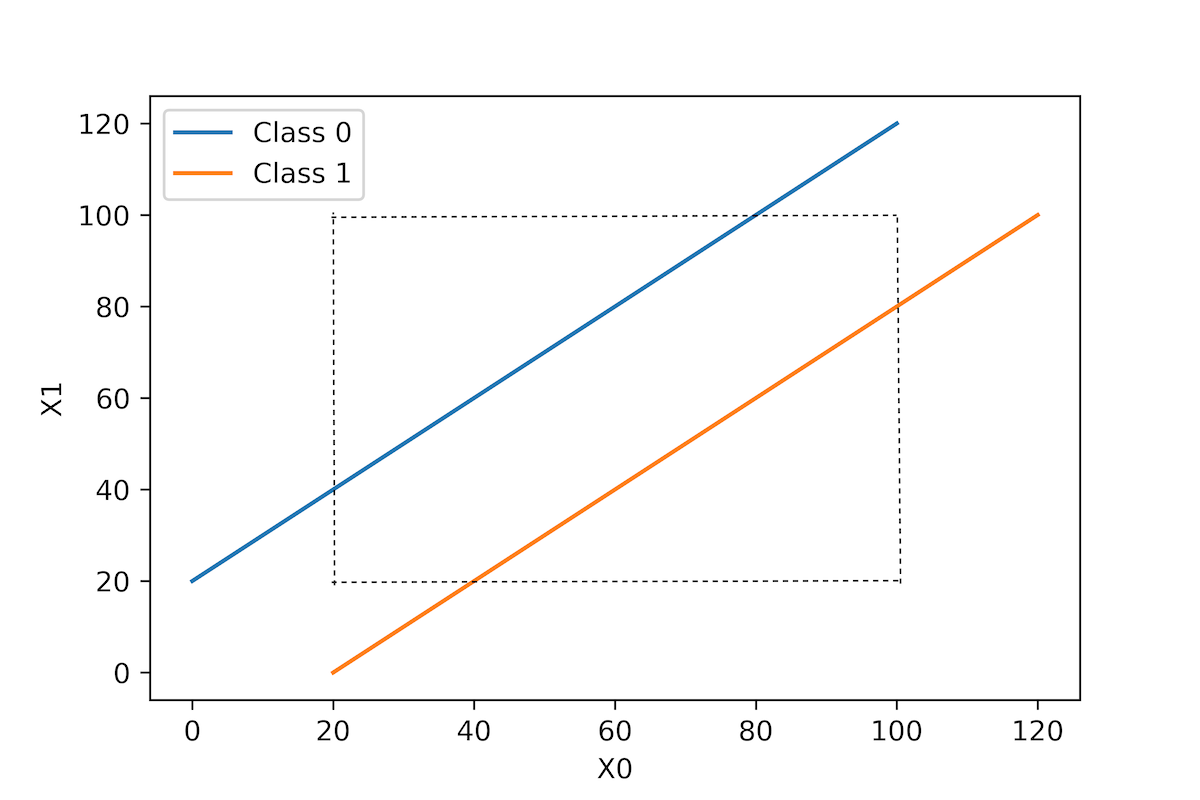
\includegraphics[scale=0.7]{Figures/simulation/example.png}
    \caption{Line Segments for the two classes}
    \label{line_segments}
\end{figure}

We express a sample data point by a tuple with $2$ entries where the first one stands for $X_0$ while the second one for $X_1$. For the simplicity of analysis, we further assume that $X_0$'s are uniformly distributed in both cases, and we can discretize $X_0$ and $X_1$ into equal bins with length $10$. Then in this way, $\mathbb{P}(X_i=x|Y=y)=0.1$ for any $i,y\in\{0,1\}$ for points with $X_0\in[20,100]$ and $X_1\in[20,100]$, i.e., the points inside the rectangle with dashed lines in Figure \ref{line_segments}, while the following cases have zero probability and require Laplacian correction in practice.
\begin{enumerate}
    \item $X_0\in[100,120]$ \textit{or} $X_1\in[0,20]$ conditioning on $Y=0$.
    \item $X_0\in[0,20]$ \textit{or} $X_1\in[100,120]$ conditioning on $Y=1$.
\end{enumerate}
Suppose we want to classify two sample points, $\mathbf{X}^{(1)}=(10,30)$ and $\mathbf{X}^{(2)}=(55,35)$. By the formulas for the two line segments, we know that $\mathbf{X}^{(1)}$ belongs to class $0$ and $\mathbf{X}^{(2)}$ belongs to class $1$. We calculate the posterior probabilities $\mathbb{P}(Y|X_0, X_1)$ using Na\"ive Bayes and CIBer, respectively as follows:
\begin{itemize}
    \item Na\"ive Bayes:
    \begin{itemize}
    \item{$\mathbf{X}^{(1)}=(10,30)$}
     \begin{equation*}
     \begin{aligned}
      \mathbb{P}(Y=0|X_0=10, X_1=30)\propto&\mathbb{P}(X_0=10,X_1=30|Y=0)\cdot\mathbb{P}(Y=0)\\
     =&\mathbb{P}(X_0=10|Y=0)\cdot\mathbb{P}(X_1=30|Y=0)\cdot\mathbb{P}(Y=0)\\
     =&0.1\cdot0.1\cdot0.5\\
     =&0.0005
     \end{aligned}
     \end{equation*}
     \begin{equation*}
     \begin{aligned}
      \mathbb{P}(Y=1|X_0=10, X_1=30)\propto&\mathbb{P}(X_0=10,X_1=30|Y=1)\cdot\mathbb{P}(Y=1)\\
     =&\mathbb{P}(X_0=10|Y=1)\cdot\mathbb{P}(X_1=30|Y=1)\cdot\mathbb{P}(Y=1)\\     
     =&0\cdot0.1\cdot0.5\\
     =&0
     \end{aligned}
     \end{equation*}

    \item{$\mathbf{X}^{(2)}=(55,35)$}
     \begin{equation*}
     \begin{aligned}
      \mathbb{P}(Y=0|X_0=55, X_1=35)\propto&\mathbb{P}(X_0=55,X_1=35|Y=0)\cdot\mathbb{P}(Y=0)\\
     =&\mathbb{P}(X_0=55|Y=0)\cdot\mathbb{P}(X_1=35|Y=0)\cdot\mathbb{P}(Y=0)\\
     =&0.1\cdot0.1\cdot0.5\\
     =&0.0005
     \end{aligned}
     \end{equation*}
     \begin{equation*}
     \begin{aligned}
      \mathbb{P}(Y=1|X_0=55, X_1=35)\propto&\mathbb{P}(X_0=55,X_1=35|Y=1)\cdot\mathbb{P}(Y=1)\\
     =&\mathbb{P}(X_0=55|Y=1)\cdot\mathbb{P}(X_1=35|Y=1)\cdot\mathbb{P}(Y=1)\\
     =&0.1\cdot0.1\cdot0.5\\
     =&0.0005
     \end{aligned}
     \end{equation*}
    \end{itemize}


    \item CIBer:
    \begin{itemize}
    \item{$\mathbf{X}^{(1)}=(10,30)$}
     \begin{equation*}
     \begin{aligned}
      \mathbb{P}(Y=0|X_0=10, X_1=30)\propto&\mathbb{P}(X_0=10,X_1=30|Y=0)\cdot \mathbb{P}(Y=0)\\
     =&Leb([0,0.1]\cap[0,0.1])\cdot0.5\\
     =&0.05
     \end{aligned}
     \end{equation*}
     \begin{equation*}
     \begin{aligned}
      \mathbb{P}(Y=1|X_0=10, X_1=30)\propto&\mathbb{P}(X_0=10,X_1=30|Y=1)\cdot\mathbb{P}(Y=1)\\
     =&Leb(\phi\cap[0.2,0.3])\cdot0.5\\
     =&0
     \end{aligned}
     \end{equation*}

    \item{$\mathbf{X}^{(2)}=(55,35)$}
     \begin{equation*}
     \begin{aligned}
      \mathbb{P}(Y=0|X_0=55, X_1=35)\propto&\mathbb{P}(X_0=55,X_1=35|Y=0)\cdot\mathbb{P}(Y=0)\\
     =&Leb([0.5,0.6]\cap[0.1,0.2])\cdot0.5\\
     =&0
     \end{aligned}
     \end{equation*}
     \begin{equation*}
     \begin{aligned}
      \mathbb{P}(Y=1|X_0=55, X_1=35)\propto&\mathbb{P}(X_0=55,X_1=35|Y=1)\cdot\mathbb{P}(Y=1)\\
     =&Leb([0.3,0.4]\cap[0.3,0.4])\cdot0.5\\
     =&0.05
     \end{aligned}
     \end{equation*}
    \end{itemize}
\end{itemize}

A classifier has no power of judgement if $\mathbb{P}(Y=0|X_0,X_1)=\mathbb{P}(Y=1|X_0,X_1)$. Thus, the calculation above indicates that Na\"ive Bayes has no power of judgement for $\mathbf{X}^{(2)}$. In general, in this example, for points in $[20,100]\times[20,100]$, since $\mathbb{P}(X_0|Y=0)=\mathbb{P}(X_0|Y=1)$ and $\mathbb{P}(X_1|Y=0)=\mathbb{P}(X_1|Y=1)$, the product of conditional joint probability and class prior probability is equal for both classes. It works well in cases like $\mathbf{X}^{(1)}$ in which the conditional marginal probability of one class is $0$. However, CIBer avoids this problem because the difference of intercepts for the two line segments makes one of the interval intersection empty, and thus placing all the weights onto the real class no matter where the point falls.

Next, we shall verify this example using a large number of simulated data points. First we shall discretize the data in three different ways, namely, discretizing into $10$ bins with equal length, discretizing by mean and standard deviation, discretizing by minimum description length principle. However, to some extent, discretization will cause information loss. Thus, in Section \ref{simulation_without_discrete}, we try to simulate much more synthetic data and make the bin sufficiently small so that the marginal density can be approximated by the empirical probability mass in the bin which contains the corresponding value. Here, for each class, we uniformly generate $5000$ samples and split out $20\%$ as testing set while the remaining as training set. Then we apply both CIBer and Na\"ive Bayes to the synthetic data and repeat the experiment for $1000$ times. The box-plots of the accuracy scores for both methods are shown in Figure \ref{with_discretize}.

\begin{figure}[!htbp]
    \includegraphics[scale=0.5]{Figures/simulation/With discretization.png}
    \caption{Accuracy Scores With Different Discretizations}
    \label{with_discretize}
\end{figure}

When applying the uniform discretization (discretizing into $10$ bins with equal length), CIBer is always as optimal as we expect and achieves an accuracy score of $1$ all the time, while for Na\"ive Bayes, the accuracy varies because of the randomness caused by points in range $[20,100]\times[20,100]$. Meanwhile, we ascribe the deterioration to the performance of CIBer in the other two discretization methods to the improper division of intervals for the two predictive features, which might have caused the empty intersections in some cases. But in general, CIBer has shown a higher accuracy and a lower variance on the synthetic data.

\subsection{Verification without discretization}\label{simulation_without_discrete}
Since discretization may cause troubles like information loss, we further extend the simulation study by synthesizing much more data points and discretize the range into sufficiently small intervals so that the probability mass of each sub-interval approximates the density. This time, we synthesize $500000$ data points for each class and take $1000$ bins for the two predictive features so that each bin contains $500$ data points on average. The experiment has been repeated for $1000$ times. The number of bins and the number of data points can be further increased to make the probability mass closer to the density but the computational efficiency will decline simultaneously. We take these amounts in order to balance this trade-off while keeping the result persuasive. The accuracy scores for CIBer and Na\"ive Bayes are shown in Figure \ref{without_discrete}. It can be seen that the accuracy of both methods becomes more stable compared to the experiments with $5000$ data points. Also, CIBer demonstrates significant superiority over Na\"ive Bayes when no typical discretization is applied.

\begin{figure}
    \centering
    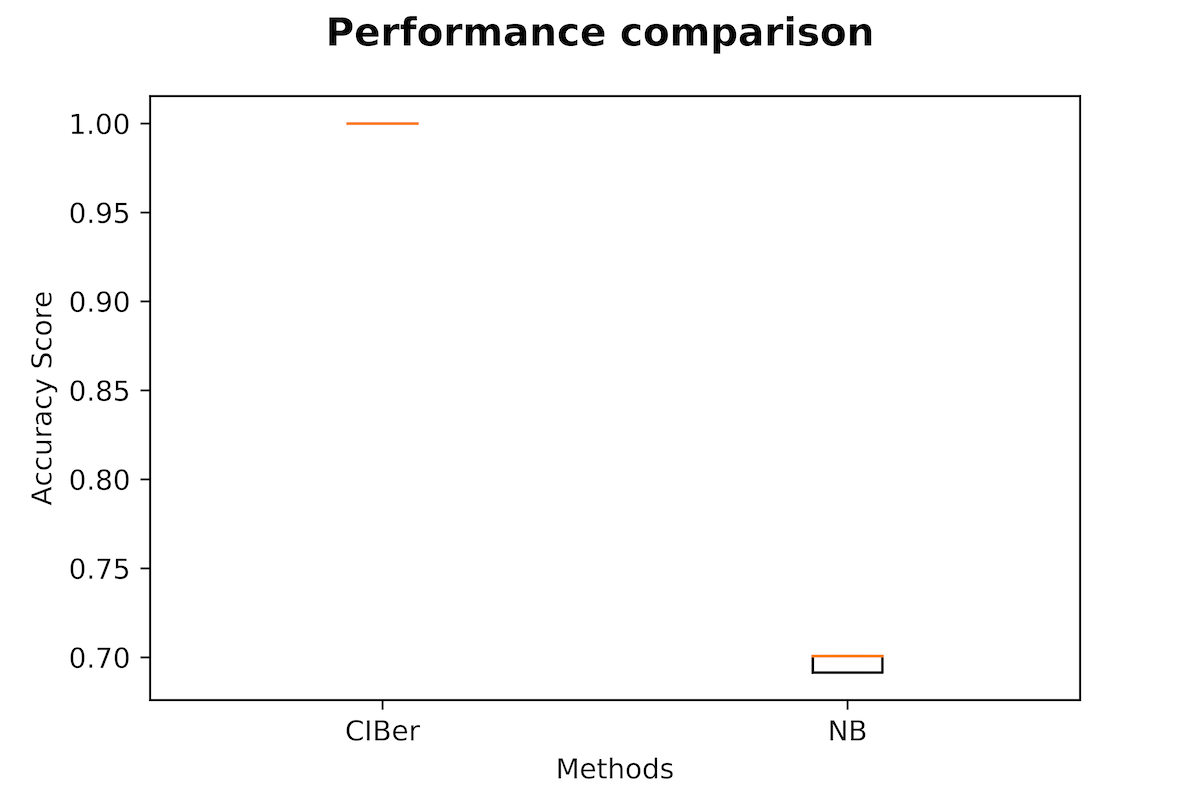
\includegraphics[scale=0.7]{Figures/simulation/sufficiently small discrete.png}
    \caption{Approximation by sufficiently small bins}
    \label{without_discrete}
\end{figure}

Hence, this further verification has confirmed our claim that discretization is applied because the limited amount of data makes it unable to use sufficiently small bins to approximate the density. Next, we shall compare the running time of CIBer and Na\"ive Bayes, and analyze the time complexity in terms of training and testing. 

\subsection{Time Complexity Analysis}
In this section, we first compare the running time of training and testing for both CIBer and Na\"ive Bayes when changing the number of predictive features. To make an intuitive comparison, we take the ratio of running time for CIBer and Na\"ive Bayes and then plot the ratios at different number of features. Later on, we analyze the theoretical time complexity and make a comparison with the simulation results. Our theoretical analysis is in accordance with the simulation results.

Unlike the previous setting of only $2$ features, here we adjust the number of features in each round. For simplicity, in each experiment, we set the number of feature pairs in the simulated data, denoted by $\lambda$. Then 

\begin{itemize}
    \item Class $0$: $X_{2i} = X_{2i-1}+20$ and $X_{2i-1}\sim U(0,100)\quad i\leq\lambda$
    \item Class $1$: $X_{2i} = X_{2i-1}-20$ and $X_{2i-1}\sim U(20,120)\quad i\leq\lambda$
\end{itemize}

Note that $X_{2i-1}{\perp\!\!\!\perp}X_{2j-1}\quad i\neq j$ in both classes. For each class, we simulate $500000$ data points and discretize the intervals into $1000$ equal-sized bins. We repeat the experiment for $10$ times for each number of feature pairs. Then we take the ratio of running time for the two models. Later on, we plot the $95\%$ confidence interval of the running time. The confidence interval of a two-tailed t-test with $9$ degrees of freedom is computed by

\begin{equation*}
    \centering
    \hat{\mu}\pm2.2622\cdot\frac{\hat{\sigma}}{\sqrt{10}}
\end{equation*}
where $\hat{\mu}$ and $\hat{\sigma}$ are the mean and standard deviation of the ratios. The relationship between the number of features and the ratio of running time is shown in Figure \ref{running_time_ratio}.

\begin{figure}[h]
\begin{tabular}{ll}
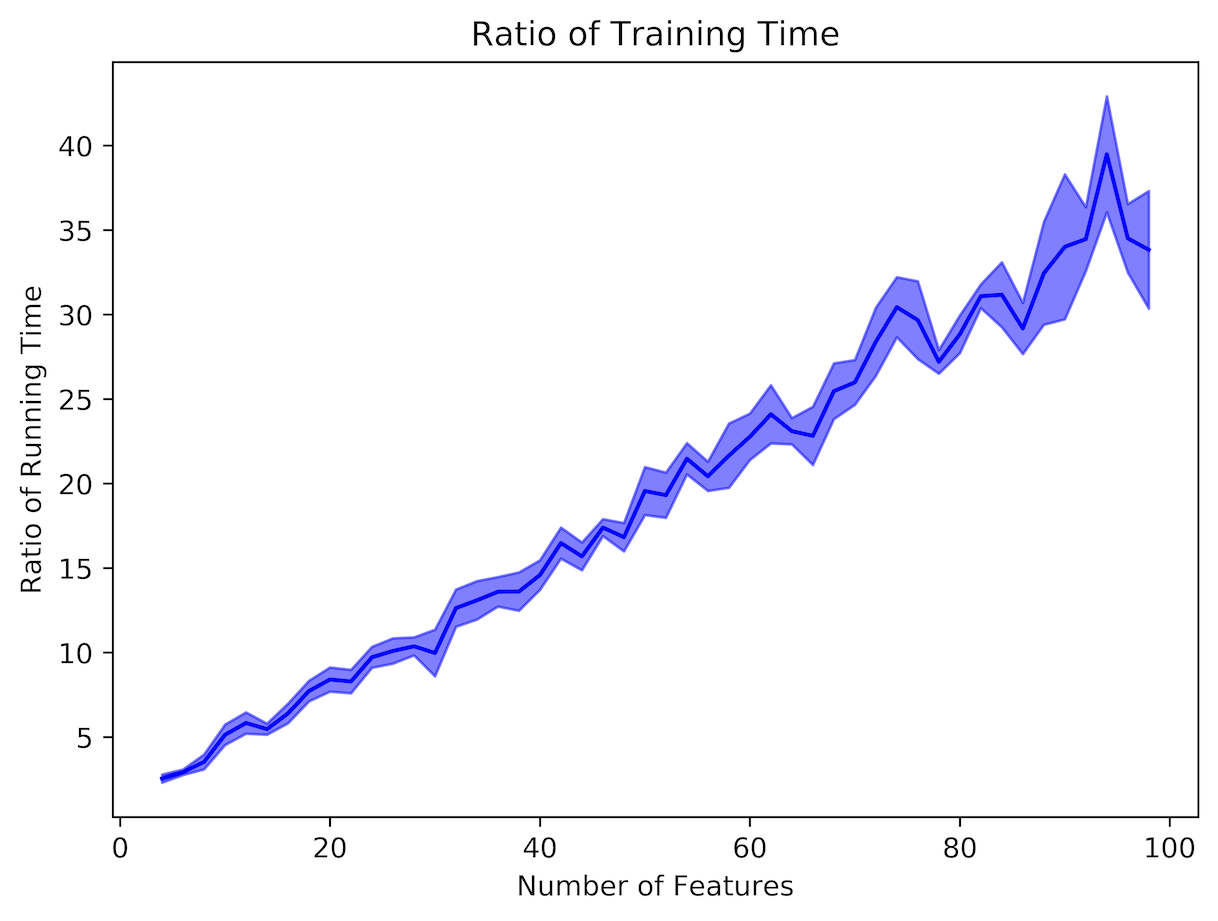
\includegraphics[scale=0.4]{Figures/simulation/training.png}
&
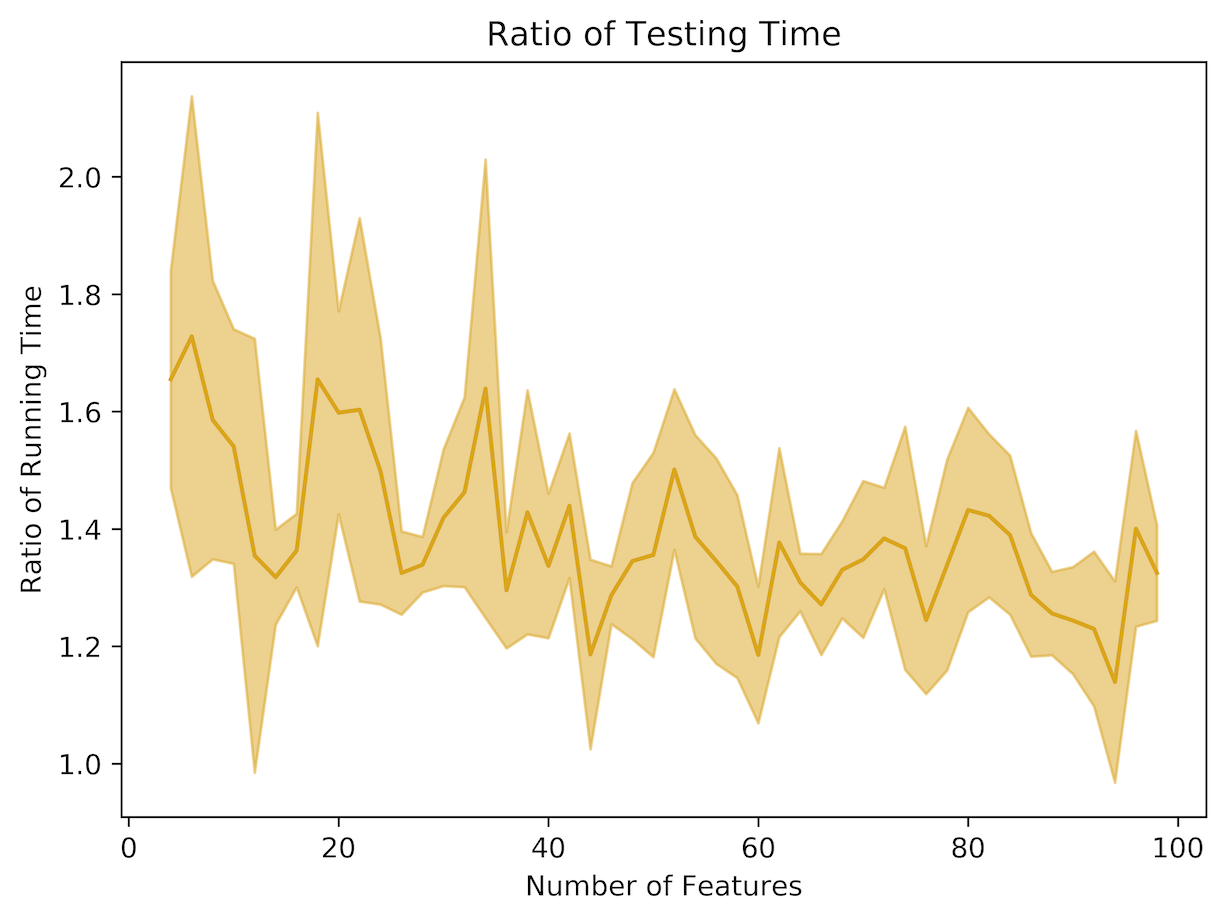
\includegraphics[scale=0.4]{Figures/simulation/testing.png}
\end{tabular}
\caption{Ratio of Running Time with 95\% Confidence Interval}
\label{running_time_ratio}
\end{figure}

We observe from the plots that, in the training process, the ratio of running time has a linear relationship with the number of features. But in the testing process, although the fluctuation becomes larger, the ratio approximately becomes a constant when adjusting the number of features. 

Next, we analyze the theoretical time complexity for both models. Our analysis is in accordance with the simulation results.

Suppose our data-set has $d$ predictive features, and the average size of sample spaces for these features is $k$. Further, we assume that there are $T$ classes in total, and for the simplicity of analysis, we assume these classes have equal prior probability. As for clustering, we assume each cluster contains $c$ features on average, and hence there should be $\frac{d}{c}$ clusters on average. Lastly, we suppose that the training set contains $n$ samples while the testing set contains $m$ samples. 

In the training process, both CIBer and Na\"ive Bayes models generate two tables. One is a one-dimensional table containing the empirical estimation of class prior probabilities. The other is a three-dimensional table containing the empirical estimation of conditional marginal probability, indexed by the class, the feature index, and the feature value \citep{zheng2005comparative}. In practice, we traverse all instances in the training set and record the occurrence of every feature value. Thus, the time complexity for filling these two tables is $O(nd)$, and the space complexity is $O(Tdk)$. Up to now, the training process for Na\"ive Bayes is done. So the training of Na\"ive Bayes costs $O(nd)$ time. But for CIBer, finding the optimal partition of features requires more time. In our heuristic method, forming the distance matrix requires the correlation coefficient matrix. There are $\binom{d}{2}$ pairs of features and time complexity for each feature pair is $O(n)$. So computing the distance matrix requires $O(nd^2)$ time. In practice, this time can be reduced by applying parallel computing. Thus, our analysis here only explains the case of \textit{serial computing}. Later on, with the help of heap, the hierarchical clustering has time complexity $O(d^2 \log d)$ \citep{kurita1991efficient}. Hence, the whole training process of CIBer has time complexity $O(d^2\cdot(n+\log d))$. In most of the cases that we have encountered, $n > \log d$. Thus, if the correlation coefficient matrix is got by serial computing, the upper bound of training complexity of CIBer is $O(nd^2)$, which should be proportional to the product of number of features and the training time of Na\"ive Bayes. Looking back to the plot for training in Figure \ref{running_time_ratio}, the linear relationship perfectly supports our analysis.

In the testing process, for each instance, Na\"ive Bayes queries from the two tables. Extracting the class prior probabilities requires $O(T)$ time, and extracting the conditional marginal probabilities requires $O(dT)$ time. Hence, it requires $O(mdT)$ time to test all the instances in the test set. As for CIBer, it takes the same amount of time to get the class prior probabilities and the conditional marginal probabilities. But for each instance conditioning on a specific class, taking the interval intersection for each cluster requires $O(c)$ time, and finding interval intersections for all clusters requires $O(d)$ time (since there are $\frac{d}{c}$ clusters on average). Thus, classifying any instance in the testing set requires $O(dT)$ time. The whole tesing procedure of CIBer has time complexity $O(mdT)$. However, since CIBer needs to compute the interval intersection, even if it does not increase the order of complexity, it costs more time than Na\"ive Bayes in reality. This explains why in the plot for testing in Figure \ref{running_time_ratio}, the ratio is always larger than $1$. But above all, the order should be the same, otherwise, the ratio should rise as the number of features increases.

\section{Empirical Evaluation}\label{empirical}
In this section, we empirically evaluate and compare the performance of multiple models on some real-world data-sets. When carrying out experiments, we choose data-sets satisfying the following principles.

\begin{itemize}
    \item Task: The task should be classification.
    \item Feature type: The features should be all numerical, or at most $1$ or $2$ categorical ones.
    \item Data type: The data should be multivariate (including multivariate time-series, but we disregard the autoregressive effects for the ease of analysis and comparation).
    \item Dimension: We prefer data-sets with tens of features so that clusters can be figured out. However, lower dimensional data-sets are also used if comonotonic structure also exists.
\end{itemize}

Since it is quite common to encounter imbalanced data-sets in classification tasks, applying the models to such data-sets directly will be very likely to result in overfitting on the majority class. In this section, when encountering imbalanced data-sets, we artificially generate synthetic data for the minority class in the training set. But for the testing set, the only operation is to scale the data using the scaler fitted on the training set. In this way, there will be no information leakeage from testing to training.

In order to investigate the generalization ability of each model, we design the experiments by changing the size of the training set and evaluate the error rate on the out-of-sample testing set. Apart from CIBer, other competitor models include Na\"ive Bayes, Decision Tree, Support Vector Machine (SVM), Logistic Regression, Random Forest, and XGBoost. Since Random Forest and XGBoost are two state-of-the-art models in machine learning but both of them incorporate the ensemble learning technique, we claim that the competitiveness of CIBer should be confirmed if its performance is about as good as or even a little bit better than these two models. Moreover, future works on the addition of ensemble learning on CIBer should increase its robustness, and hence, enhance its performance. Since the features are all numerical and the data is scaled before passing into the models, in order to provide a benchmark for the model performance, we use Gaussian Na\"ive Bayes in all the experiments.

Moreover, we also establish a case study on financial distress prediction by applying CIBer on a data-set consisting of tens of financial and non-financial characteristics of companies which later on either worked well or went bankrupt. We shall delve deeper into the clusters of features formed by CIBer and investigate the patterns revealed by the features within clusters which might have contributed to the success in bankruptcy classification. 

\subsection{Example Data-sets \& Results}
Here we introduce four different data-sets we have used for the performance comparison. The Ozone, Sensorless Diagnosis, and Glass Identification data-sets are from the Machine Learning repository of University of California, Irvine (UCI ML) \citep{Dua:2019}. The other one is the Oil Spill data-set \citep{kubat1998machine}. On each data-set, we use stratified sampling to split out a proportion of the instances as testing set and the remaining as the complete training set. In each round, we sub-sample a portion of the complete training set as the actual training set to fit the models. Since ensemble learning models sample the data from the training set with replacement, and then feed it into each weak classifier, in order to provide some insight to future work about the addition of ensemble learning on CIBer, we draw samples from the complete training set \textit{with replacement} when constructing the actual training set. Hence, even when the size of the training set reaches the maximum, the actual training sets differ in different repetitions. After fitting the models, we obtain the error rate on the testing set, and repeat such ``sub-sampling $\rightarrow$ fitting $\rightarrow$ testing'' process for $10$ times. The portion is gradually increased until the complete training set is totally used. Later, we conduct a two-tailed t-test to the error rates at each size of the training set, and obtain a $95\%$ confidence interval with $9$ degrees of freedom. The confidence interval is calculated by:
\begin{equation*}
    \hat{\mu}\pm2.262\cdot\frac{\hat{\sigma}}{\sqrt{10}}
\end{equation*}
where $\hat{\mu}$ and $\hat{\sigma}$ are the mean and standard deviation of the error rates.

The results for each method are plotted for comparison. For the convenience of viewing, in the first and second data-set, we separate the plot of results on each data-set into two subplots where the left plot shows CIBer, Na\"ive Bayes, XGBoost, and Random Forest, and the right plot shows CIBer, Decision Tree, SVM, and Logistic Regression. But for the third and fourth data-sets, there is much intersection among the bands for CIBer, random forest, and XGBoost. We further separate out the bands for random forest and XGBoost for the convenience of comparison. 

\subsubsection{Ozone Data-set}
In the Ozone data-set, each sample is a record of $72$ continuous meteorological features on a single day between $1998$ and $2004$ at the Houston, Galveston and Brazoria area. Thus, there are roughly $2500$ instances where each one represents the observation in one day within the $7$ years \citep{zhang2008forecasting}. The target variable has binary outcomes indicating whether this day was an ozone day or not. This data-set can be found at UCI ML. We split out $30\%$ as the testing set, and the remaining $70\%$ as the complete training set. The plots of the error rate change when adjusting the size of the actual training set is shown in Figure \ref{Fig_ozone}.

\begin{figure}[h]
\begin{tabular}{ll}
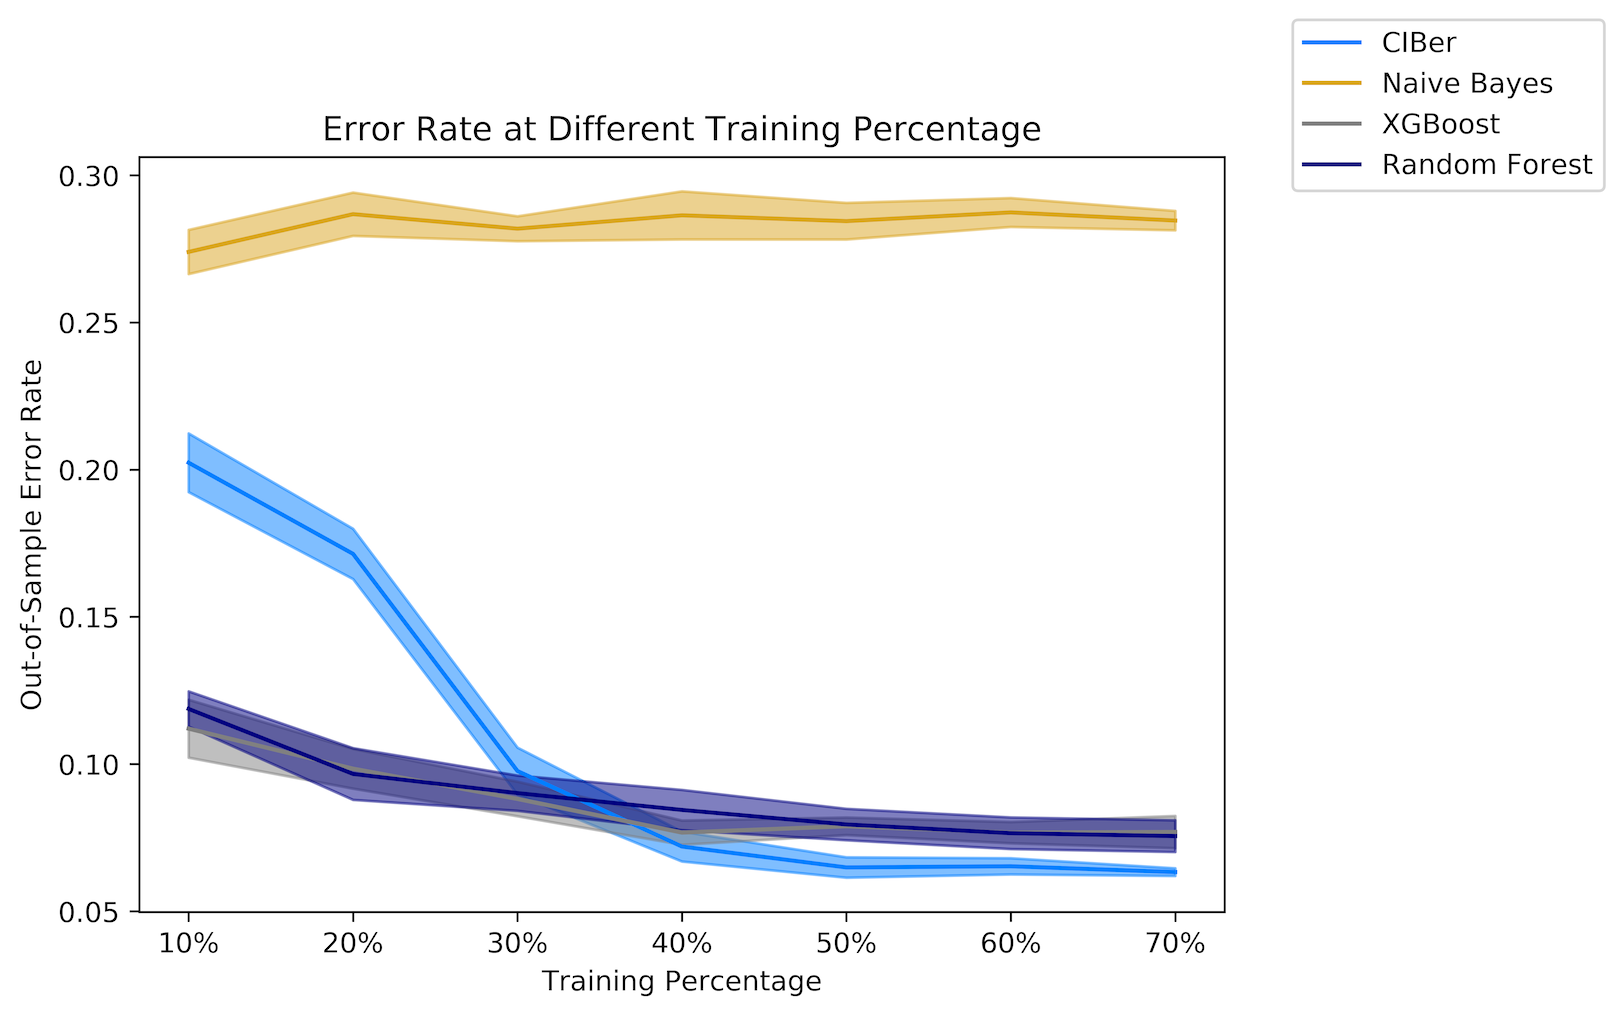
\includegraphics[width=0.5\linewidth]{Figures/Empirical/err_change_ozone_1.png}
&
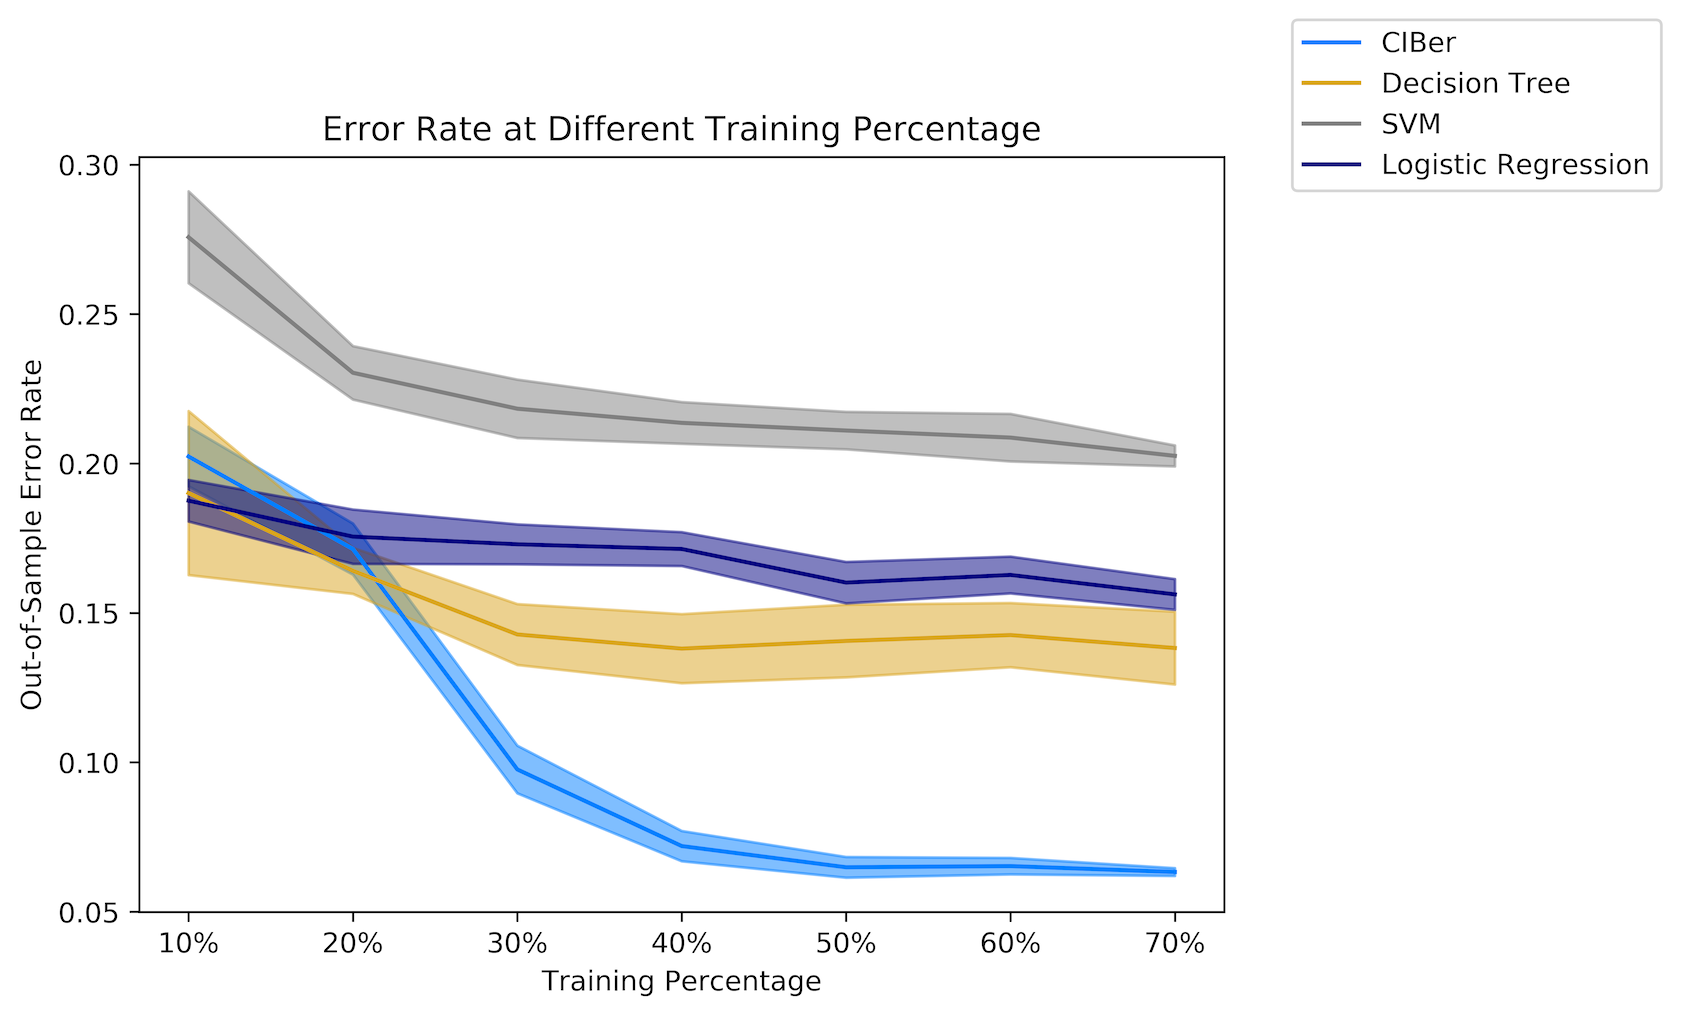
\includegraphics[width=0.5\linewidth]{Figures/Empirical/err_change_ozone_2.png}
\end{tabular}
\caption{Change of Error Rate, Ozone Data-set}
\label{Fig_ozone}
\end{figure}

It is observed that the error rates of all models except Na\"ive Bayes decrease in different scales when gradually enlarging the training set, among which CIBer decreases the most. However, as for the band of Na\"ive Bayes, although it narrows when the training set becomes larger, it keeps at a high level all the time. This should be due to the fact that Gaussian Na\"ive Bayes has already been fitted well even with a small amount of data. After all, only the sample mean and variance need to be determined. 

To some extent, CIBer is more sensitive to the amount of training data in this data-set. We ascribe such sensitivity to the fact that when the training data is far too limited, the occurrence of each feature value also becomes so limited that the variance of conditional marginal probability increases. However, when we gradually increase the amount of training data, each conditional marginal probability converges to the real one by the law of large numbers. Thus, the error rate tends to be stable when the portion of training data is larger than $40\%$. Meanwhile, CIBer achieves an even better performance than XGBoost and Random Forest when the training size goes larger. Moreover, the tapering blue band indicates that the confidence interval for the average accuracy of CIBer becomes smaller, and thus, the variance of performance becomes smaller when we increase the training size.

\subsubsection{Sensorless Drive Diagnosis Data-set}
In the Sensorless Drive Diagnosis data-set, there are $48$ features extracted from electric current drive signals. Since the drive contains both intact and defective components, with the measurement conducted for multiple times by different operating conditions, there are $11$ different classes for the instances. As for the features, the first three intrinsic mode functions of the two phase currents and their residuals were used. They are further broken down into sub-sequences, and for each subsequence, the mean, standard deviation, skewness and kurtosis were computed. Hence, it results in $48$ predictive features. The data-set is available from UCI ML. As the original data-set has over $50000$ instances, preliminary experiments have shown that even less than $10\%$ of the data is enough to fit most of the models. Thus, in order to visualize the convergence of testing accuracy while save computation time, we split out $80\%$ of the whole data-set as the testing set while the remaining $20\%$ as the complete training set. We take $10$ different training set sizes and compare the testing error rates. The plots of the error rate change are shown in Figure \ref{Fig_sensorless}.

\begin{figure}[h]
\begin{tabular}{ll}
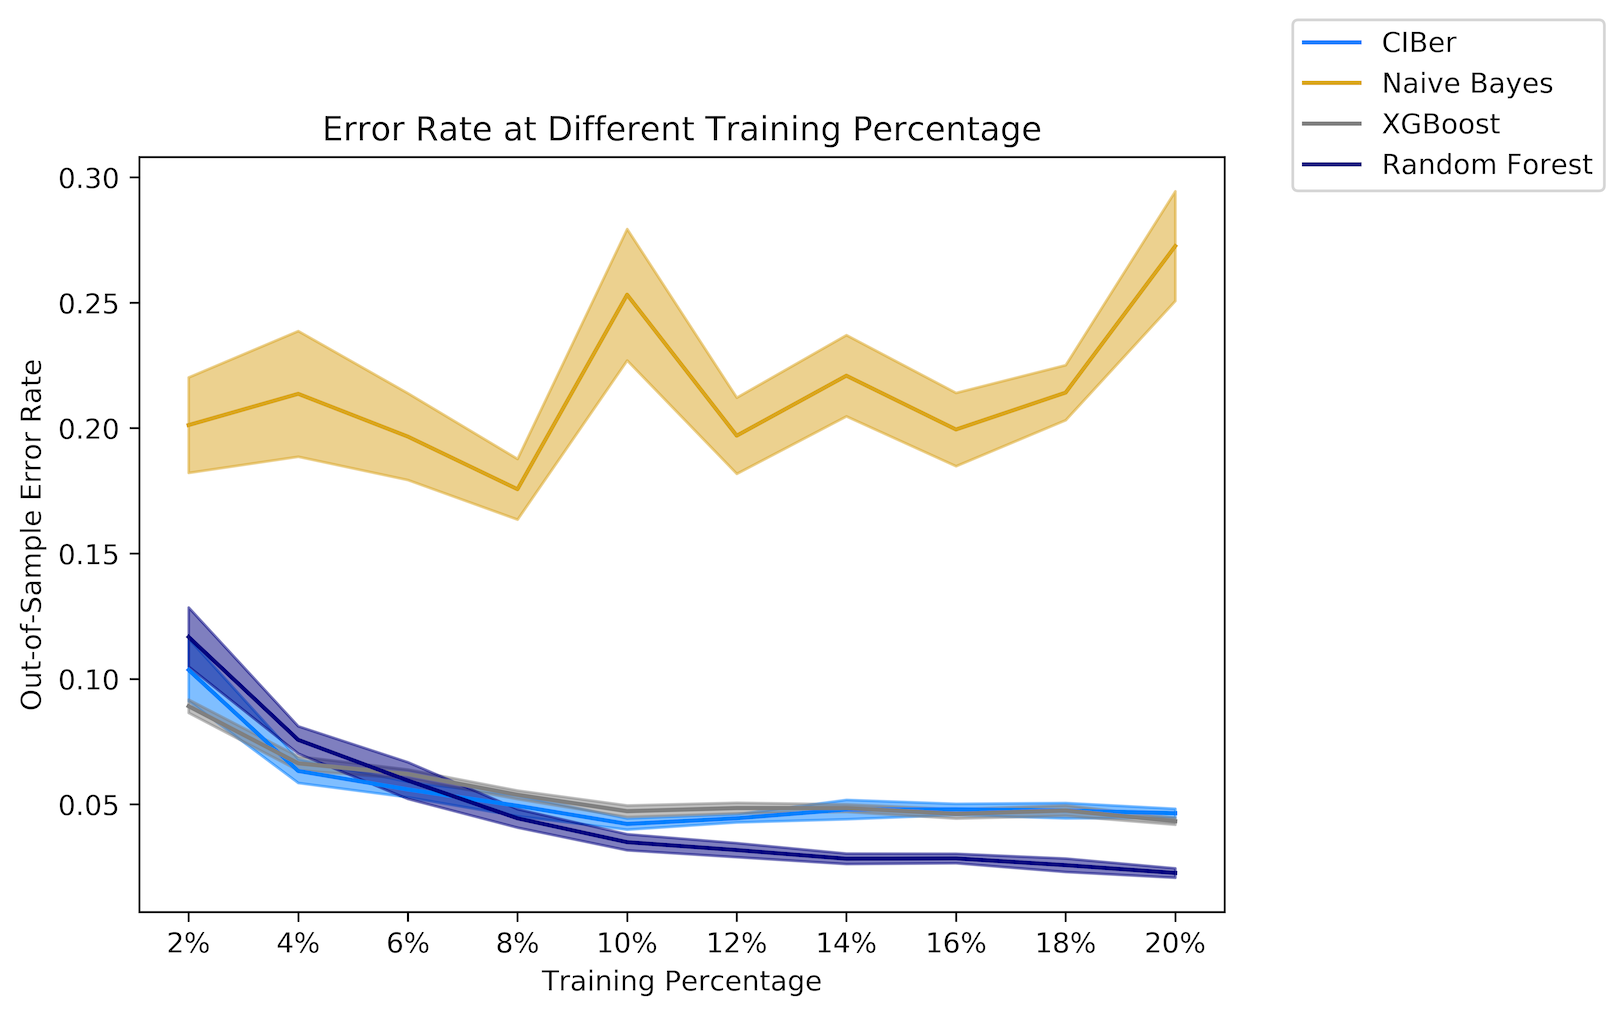
\includegraphics[width=0.5\linewidth]{Figures/Empirical/err_change_sensorless_1.png}
&
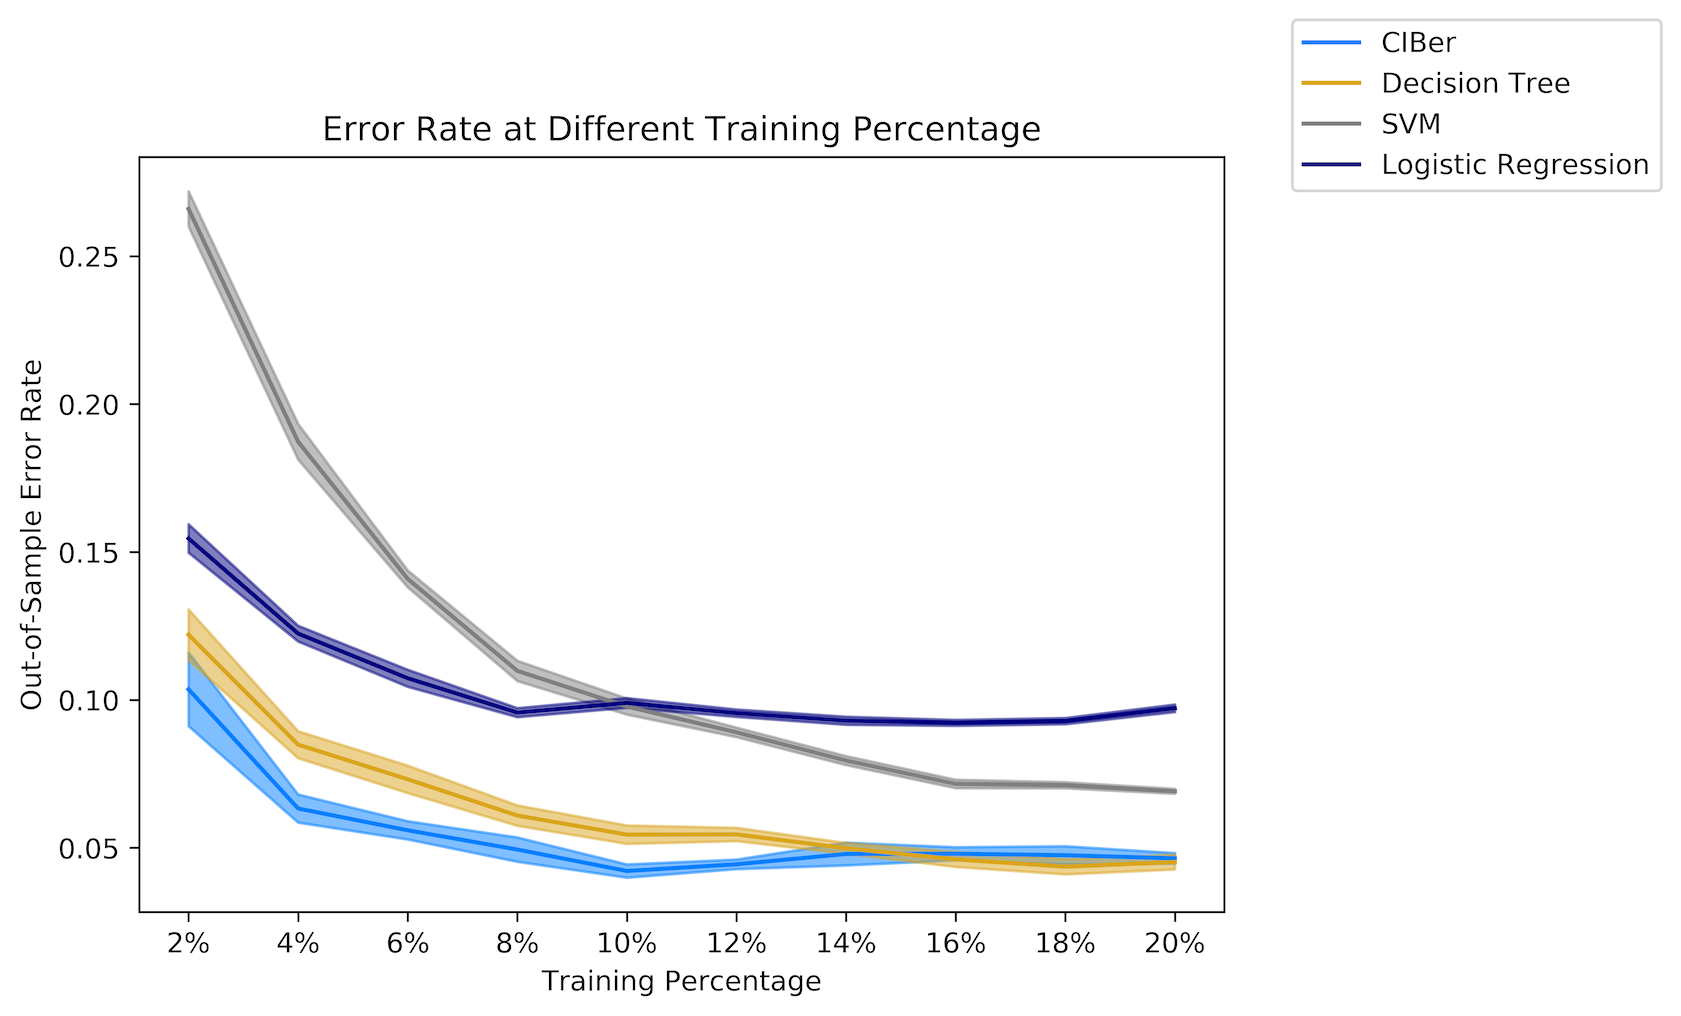
\includegraphics[width=0.5\linewidth]{Figures/Empirical/err_change_sensorless_2.png}
\end{tabular}
\caption{Change of Error Rate, Sensorless Drive Diagnosis Data-set}
\label{Fig_sensorless}
\end{figure}

In general, CIBer's performance is close to XGBoost on this data-set. Although its error rate is a bit larger than Random Forest when the training set size approaches $20\%$, it outperforms Random Forest when the training set size is small. In the right sub-plot, the performance of CIBer and Decision Tree nearly converge to the same level, and they are both better than SVM and Logistic Regression. Hence, when it comes to multiclass classification, CIBer is still competitive as the state-of-the-art models.  

\subsubsection{Oil Spill Data-set}
In the Oil Spill data-set, each sample, consisting of $48$ continuous features, is the output from a computer vision model taking raw pixel images as input. The raw pixel images were taken by radars on satellites for the detection of oil spills in the ocean. Thus, the target variable has binary outcomes indicating whether there exists oil spills or not. Since we do not have access to the original program for image processing, the only things we rely on are the extracted features in the data-set. The plots of the error rate change when adjusting the size of training set is shown in Figure \ref{Fig_oil_spill}.

\begin{figure}[ht]
  \begin{minipage}[b]{0.5\linewidth}
    \centering
    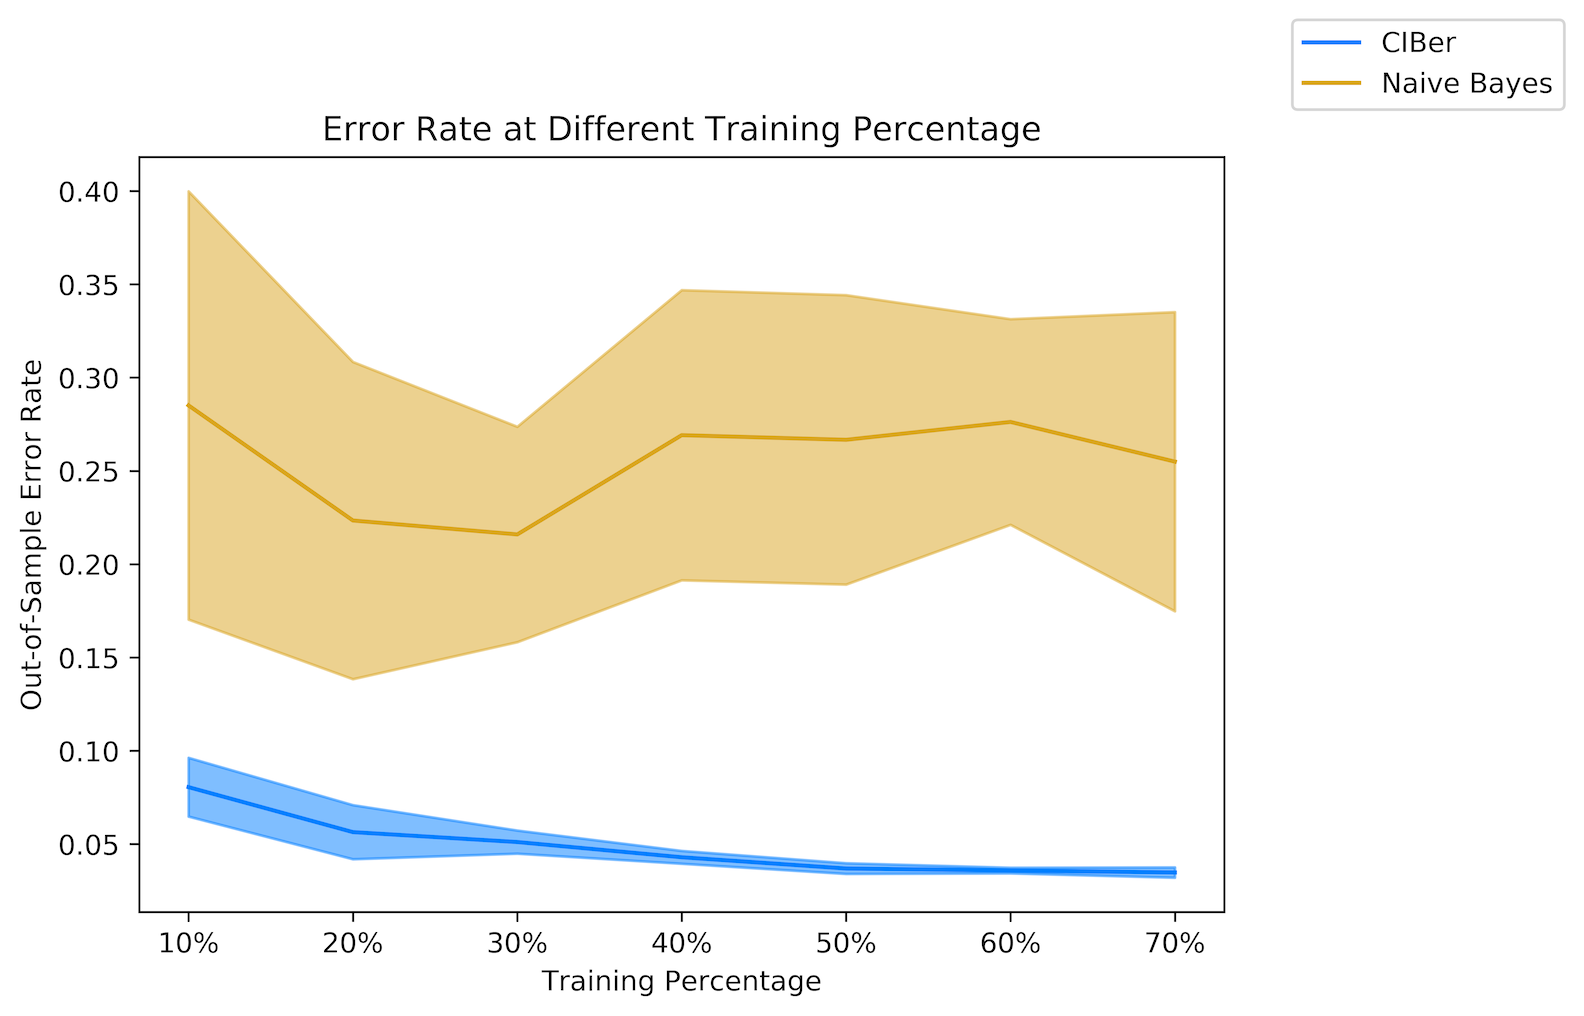
\includegraphics[width=0.85\linewidth]{Figures/Empirical/err_change_oil_1.png}
  \end{minipage}
  \begin{minipage}[b]{0.5\linewidth}
    \centering
    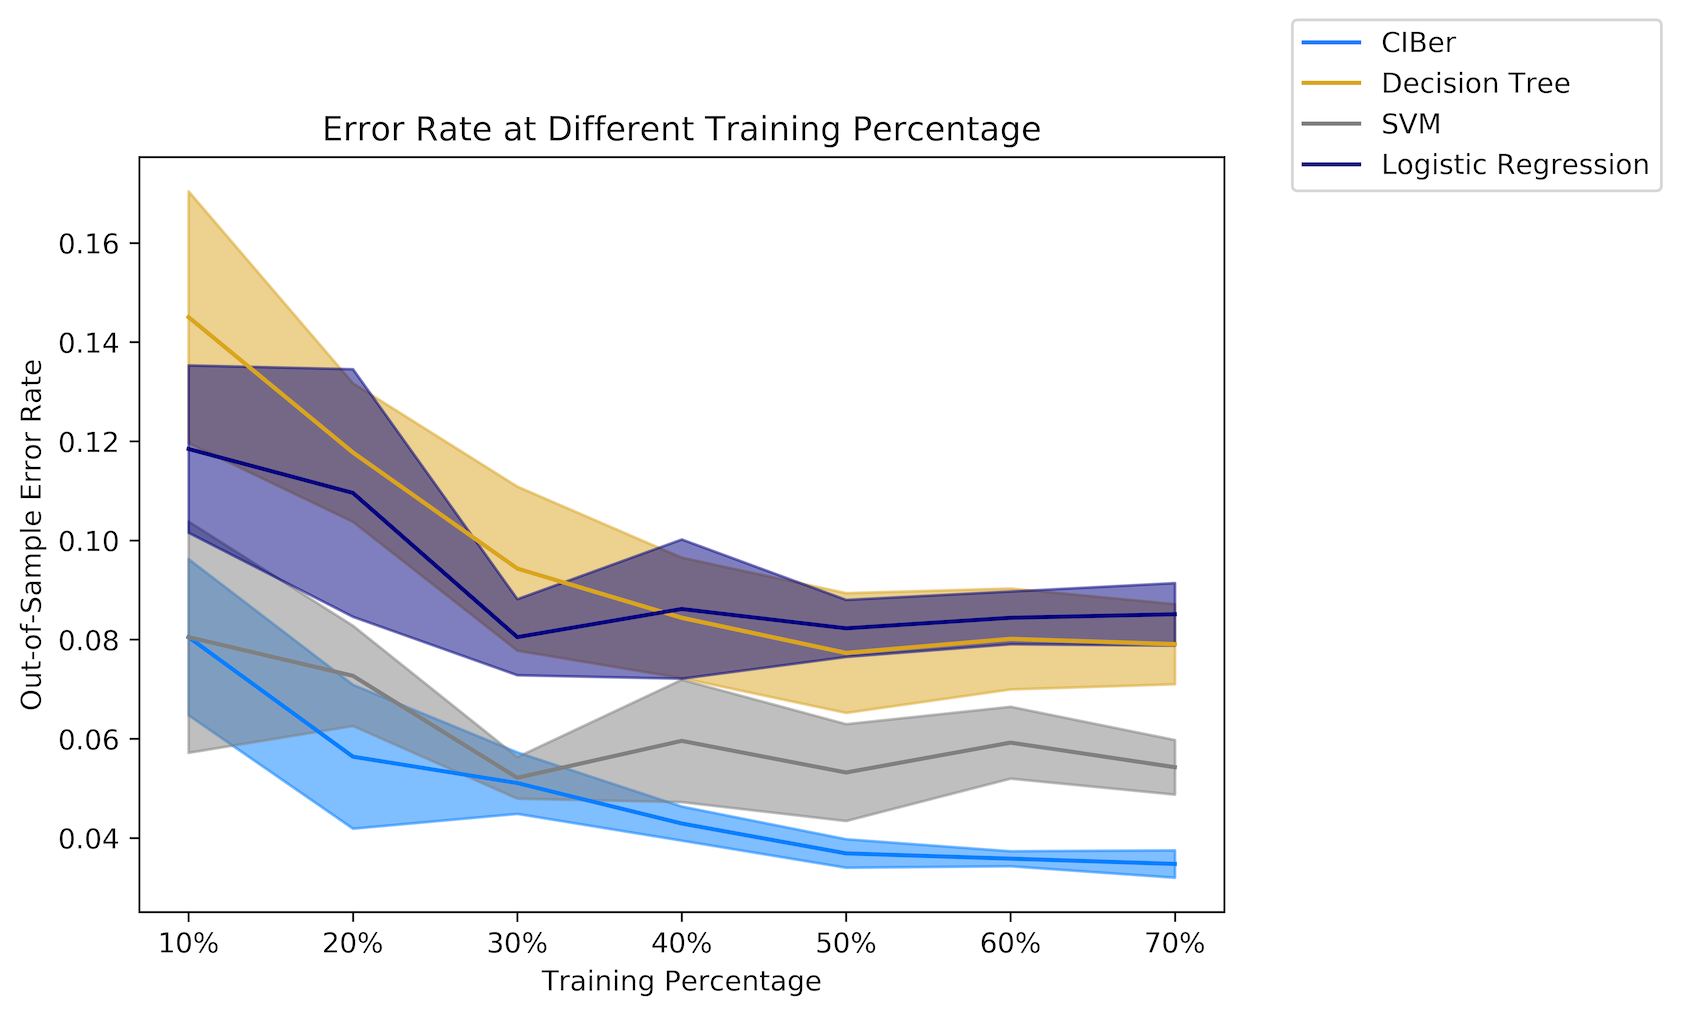
\includegraphics[width=0.9\linewidth]{Figures/Empirical/err_change_oil_2.png}
  \end{minipage} 
  \begin{minipage}[b]{0.5\linewidth}
    \centering
    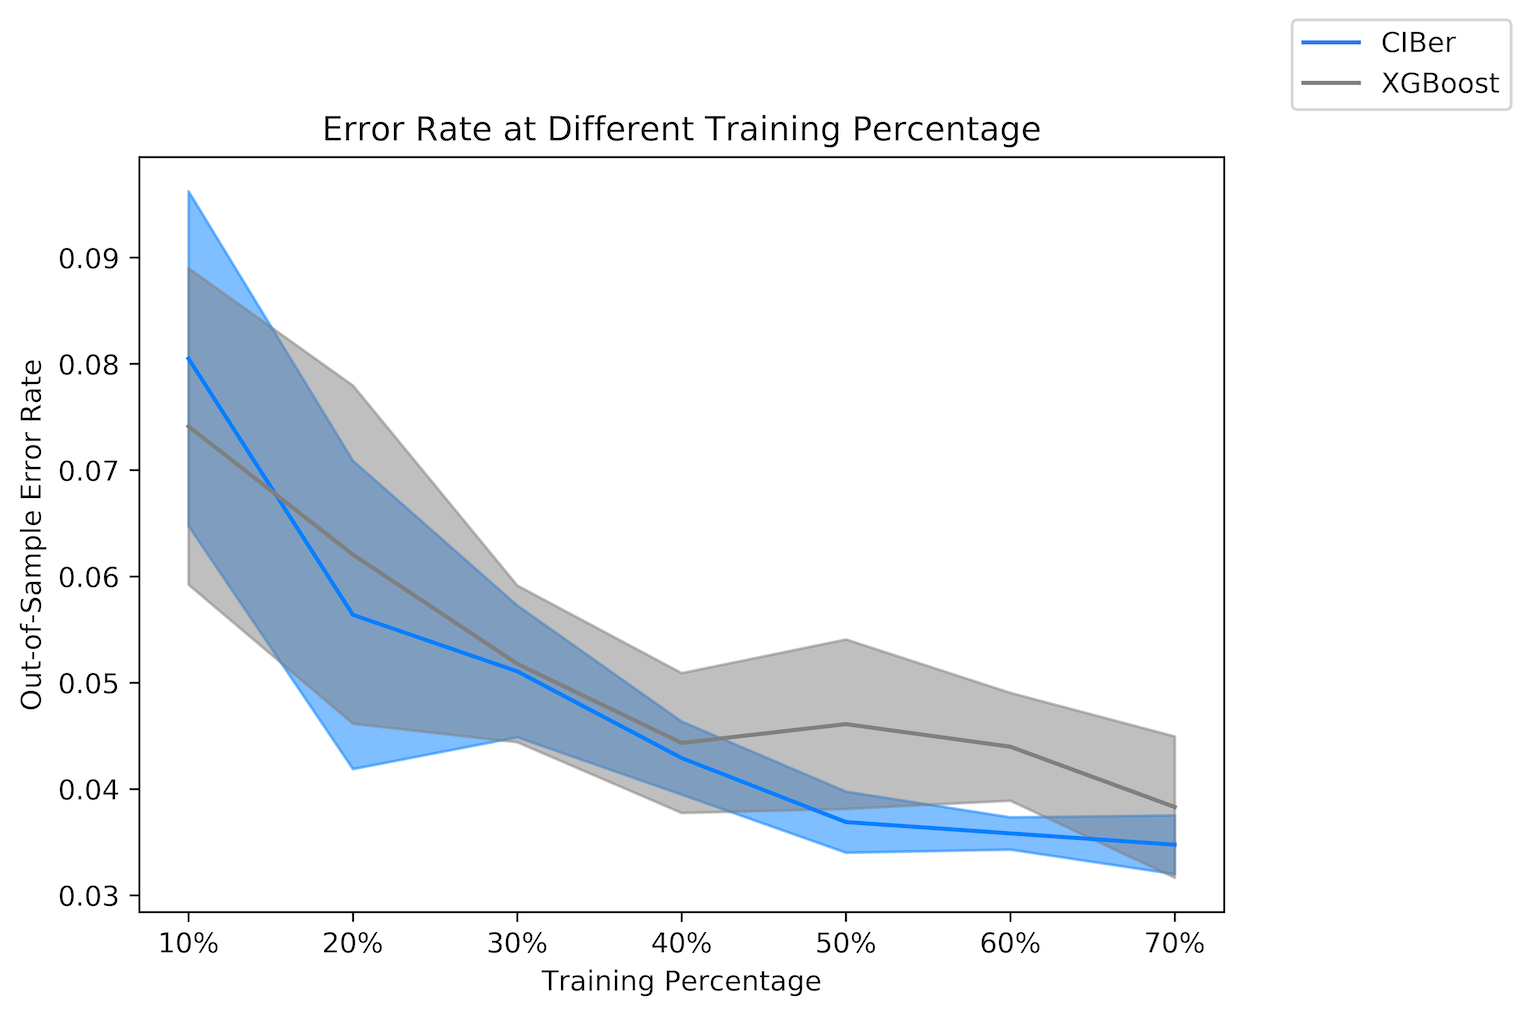
\includegraphics[width=0.85\linewidth]{Figures/Empirical/err_change_oil_xgb.png}
  \end{minipage}
  \begin{minipage}[b]{0.5\linewidth}
    \centering
    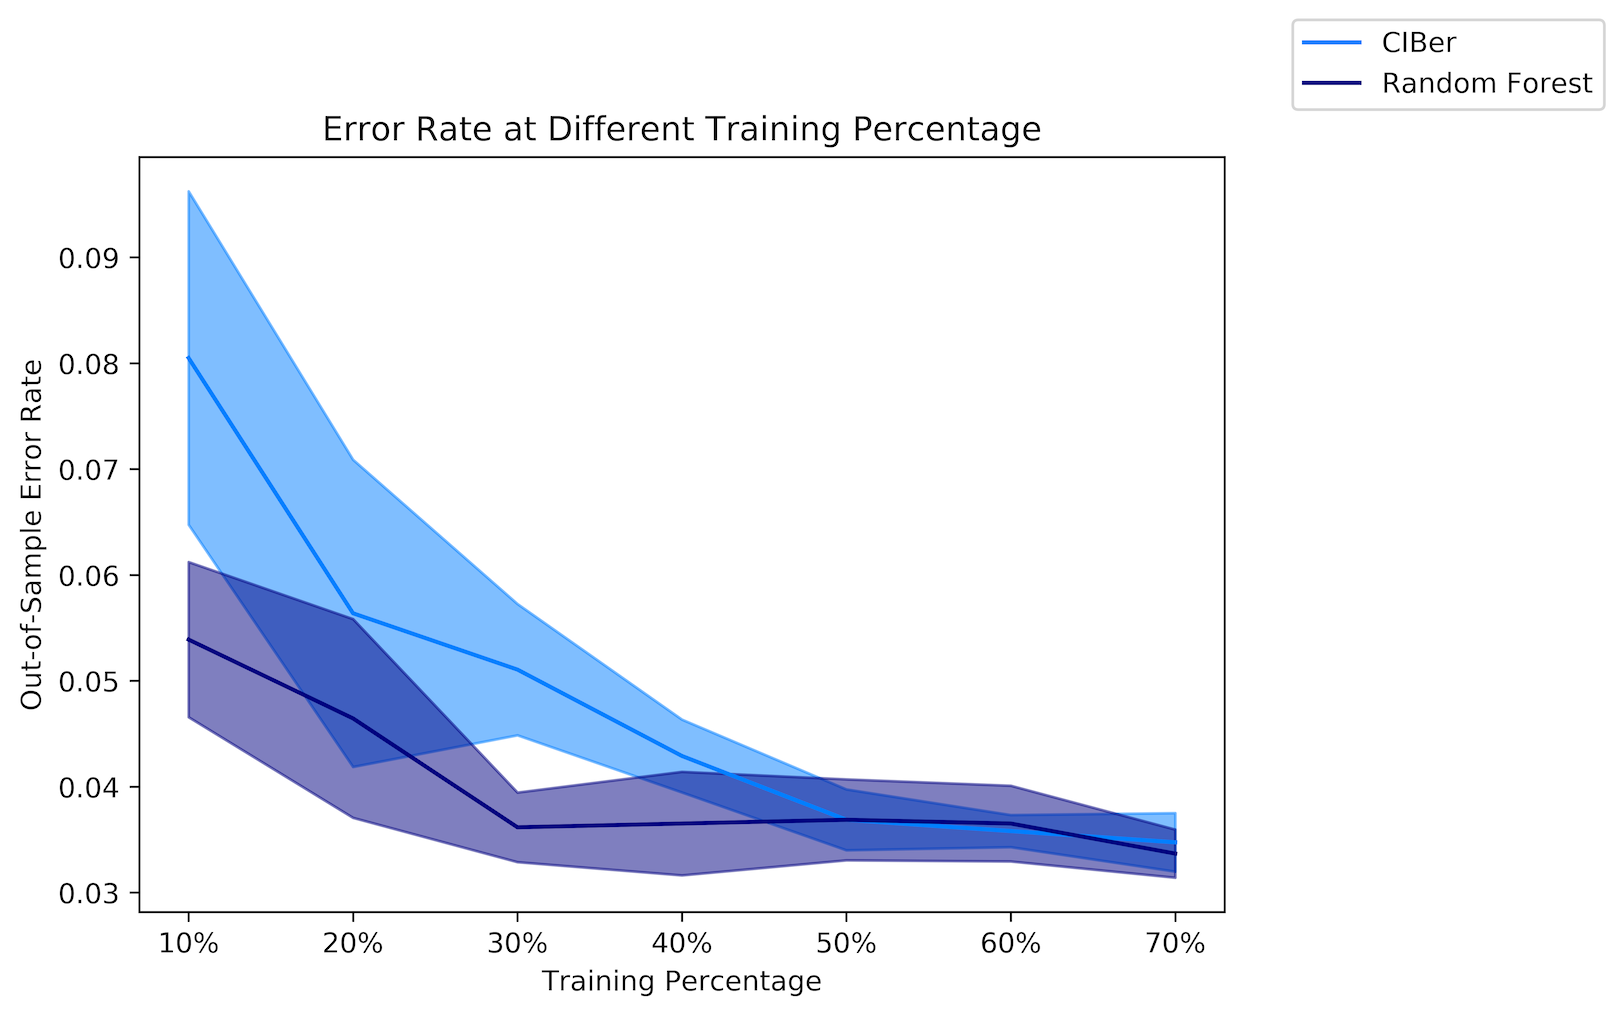
\includegraphics[width=0.9\linewidth]{Figures/Empirical/err_change_oil_rf.png}
  \end{minipage} 
  \caption{Change of Error Rate, Oil Spill Data-set} 
  \label{Fig_oil_spill}
\end{figure}

It is so clear in the upper right sub-plot that CIBer outperforms Decision Tree, SVM, and Logistic Regression not only in average error rate but also in performance stability at every training percentage. Since there is much intersection among the bands for CIBer, XGBoost, and random forest, we separate them into different sub-plots. As for the sub-plots at the lower left and lower right, we observe that CIBer has a more stable performance than the two state-of-the-art models especially XGBoost since its band-width is always smaller when the training percentage exceeds $40\%$. In terms of error rates, CIBer is always lower than XGBoost, while remains approximately the same as random forest when the training percentage exceeds $50\%$. When it comes to the scale of performance change, unlike the experiment on the Ozone data-set, this time CIBer keeps the performance at a high level all the time. The distinction in CIBer's generalization ability on different data-sets should be the consequence of the difference in data distributions. Especially, when some continuous features can just be discretized into a few bins before satisfying the minimum description length principle, it becomes much easier to capture the discrete distribution by just a small amount of data while keeping the predictability. 


\subsubsection{Glass Identification Data-set}
The size of the Glass Identification data-set is much smaller than the previous three data-sets. There are just around $200$ samples in this data-set. Each sample consists of the refractive index, and the contents of $8$ chemical elements including sodium, magnesium, aluminum, silicon, potassium, calcium, barium and iron. Meanwhile, there are $7$ classes in total representing the types of glass. The data-set is available at UCI ML. The plots of the error rate change when adjusting the percentage of training set is shown in Figure \ref{Fig_glass}. For the ease of observation and comparison, we separate out the plots for XGBoost and random forest. 

\begin{figure}[ht] 
  \begin{minipage}[b]{0.5\linewidth}
    \centering
    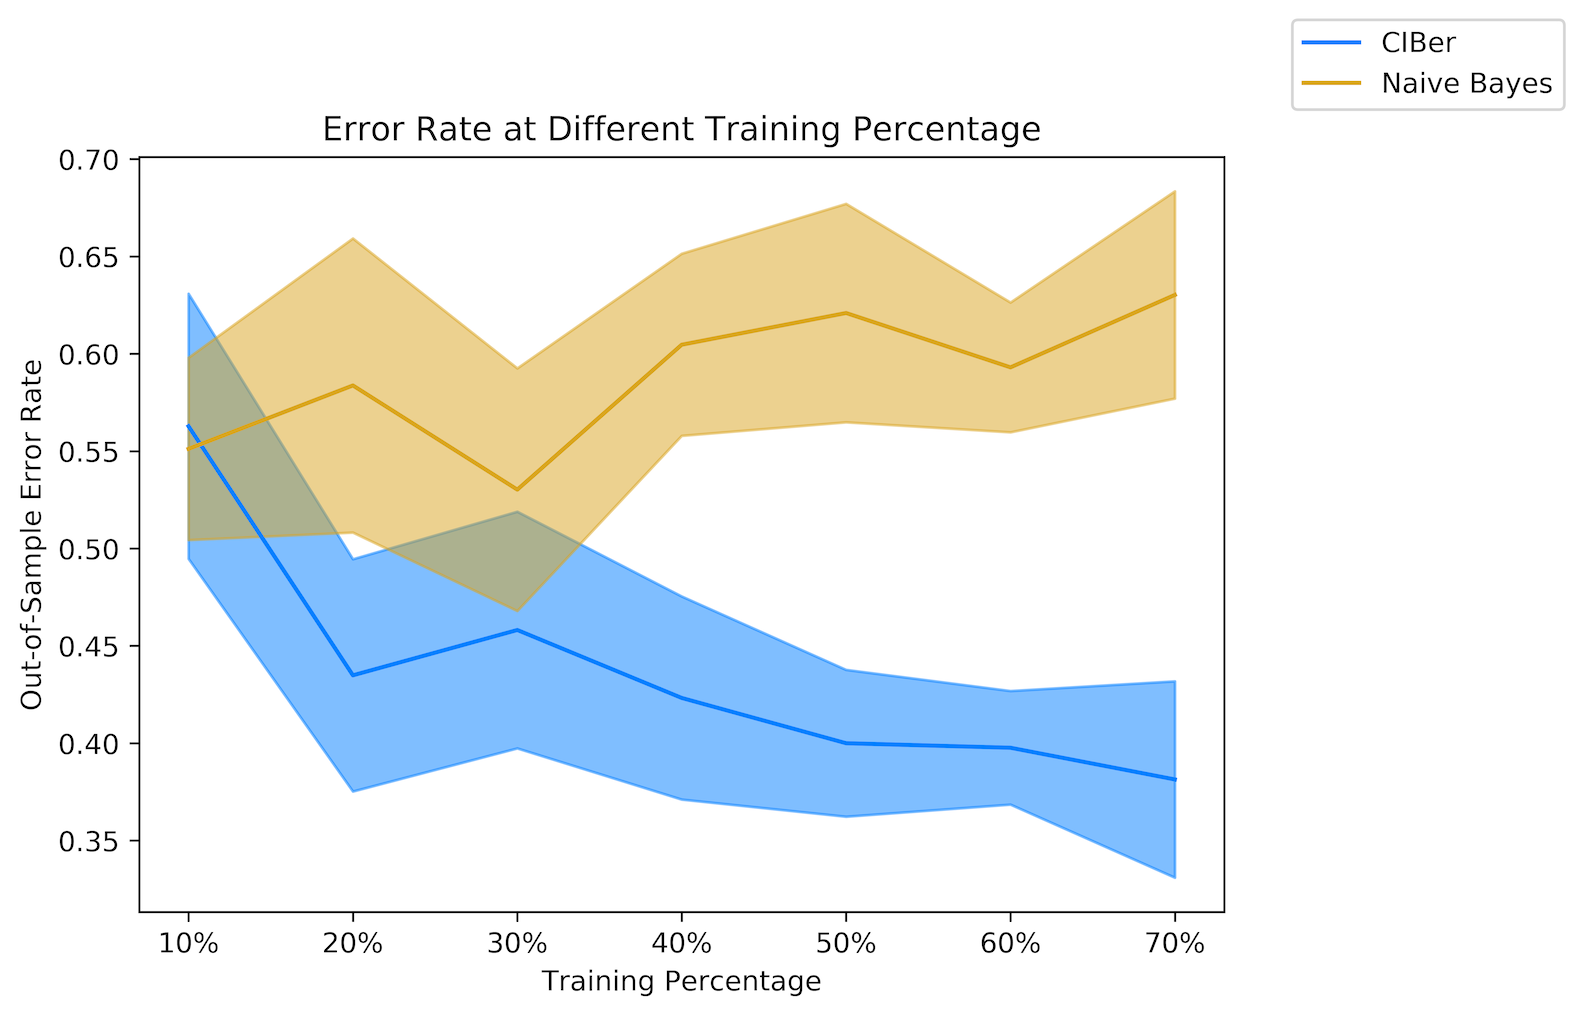
\includegraphics[width=0.85\linewidth]{Figures/Empirical/err_change_glass_1.png}
  \end{minipage}
  \begin{minipage}[b]{0.5\linewidth}
    \centering
    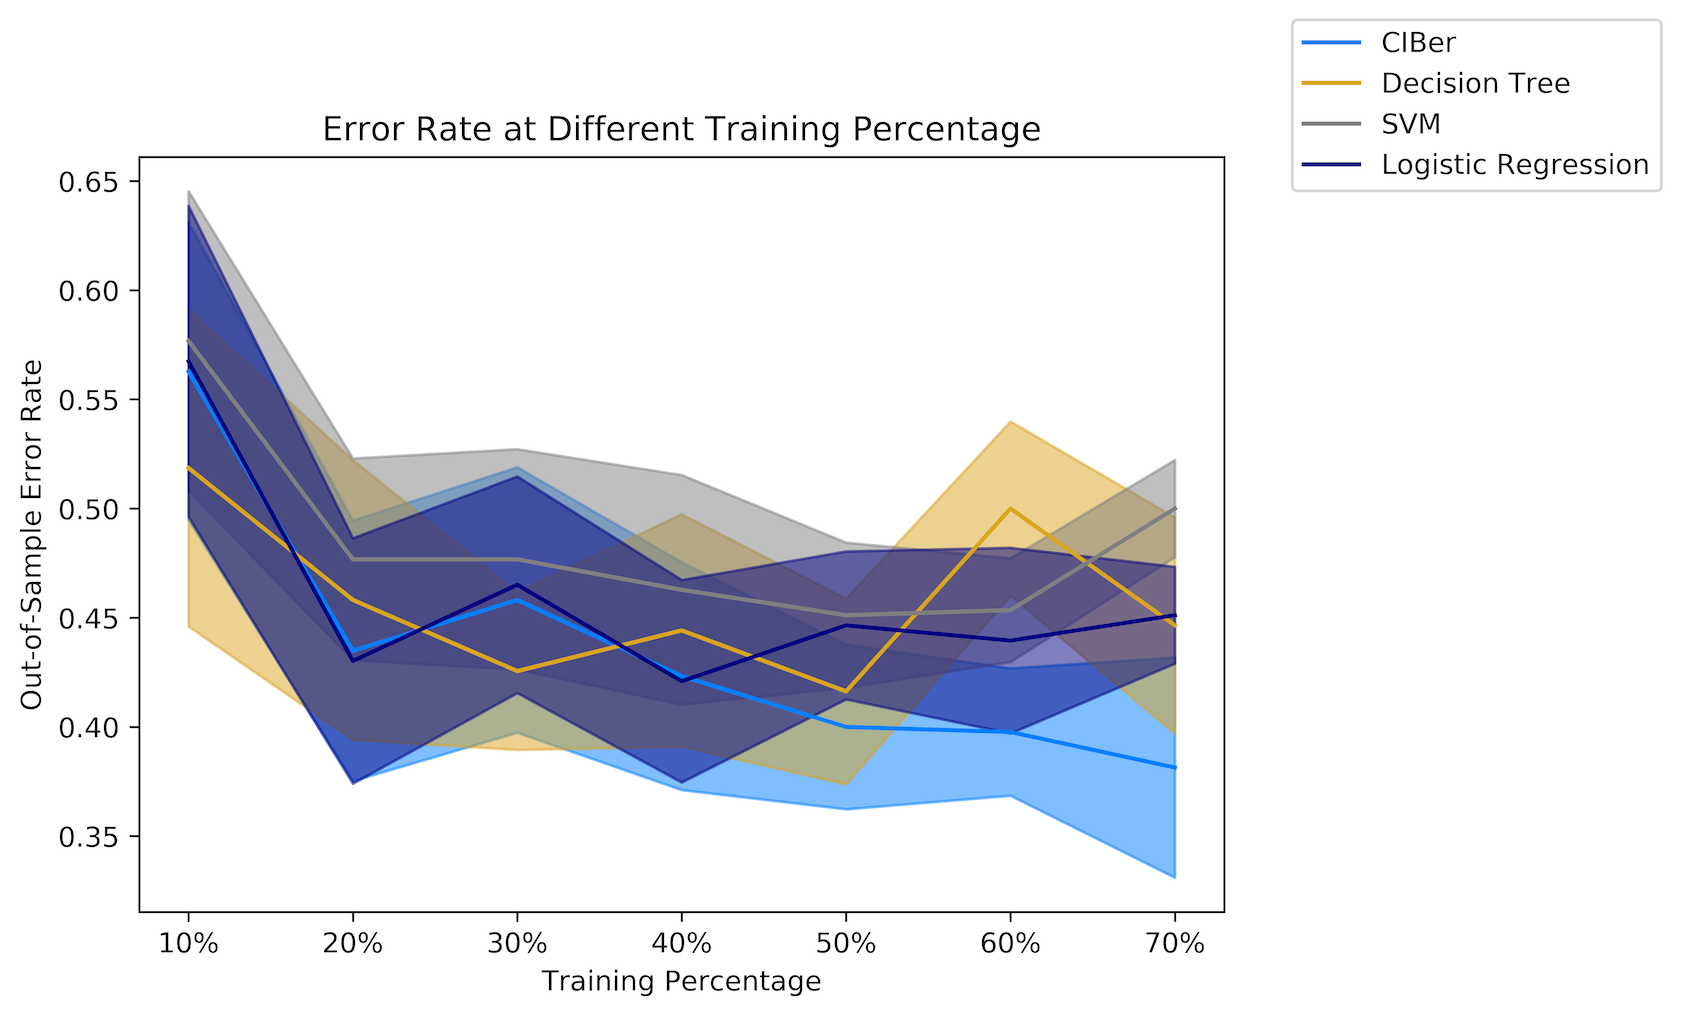
\includegraphics[width=0.9\linewidth]{Figures/Empirical/err_change_glass_2.png}
  \end{minipage} 
  \begin{minipage}[b]{0.5\linewidth}
    \centering
    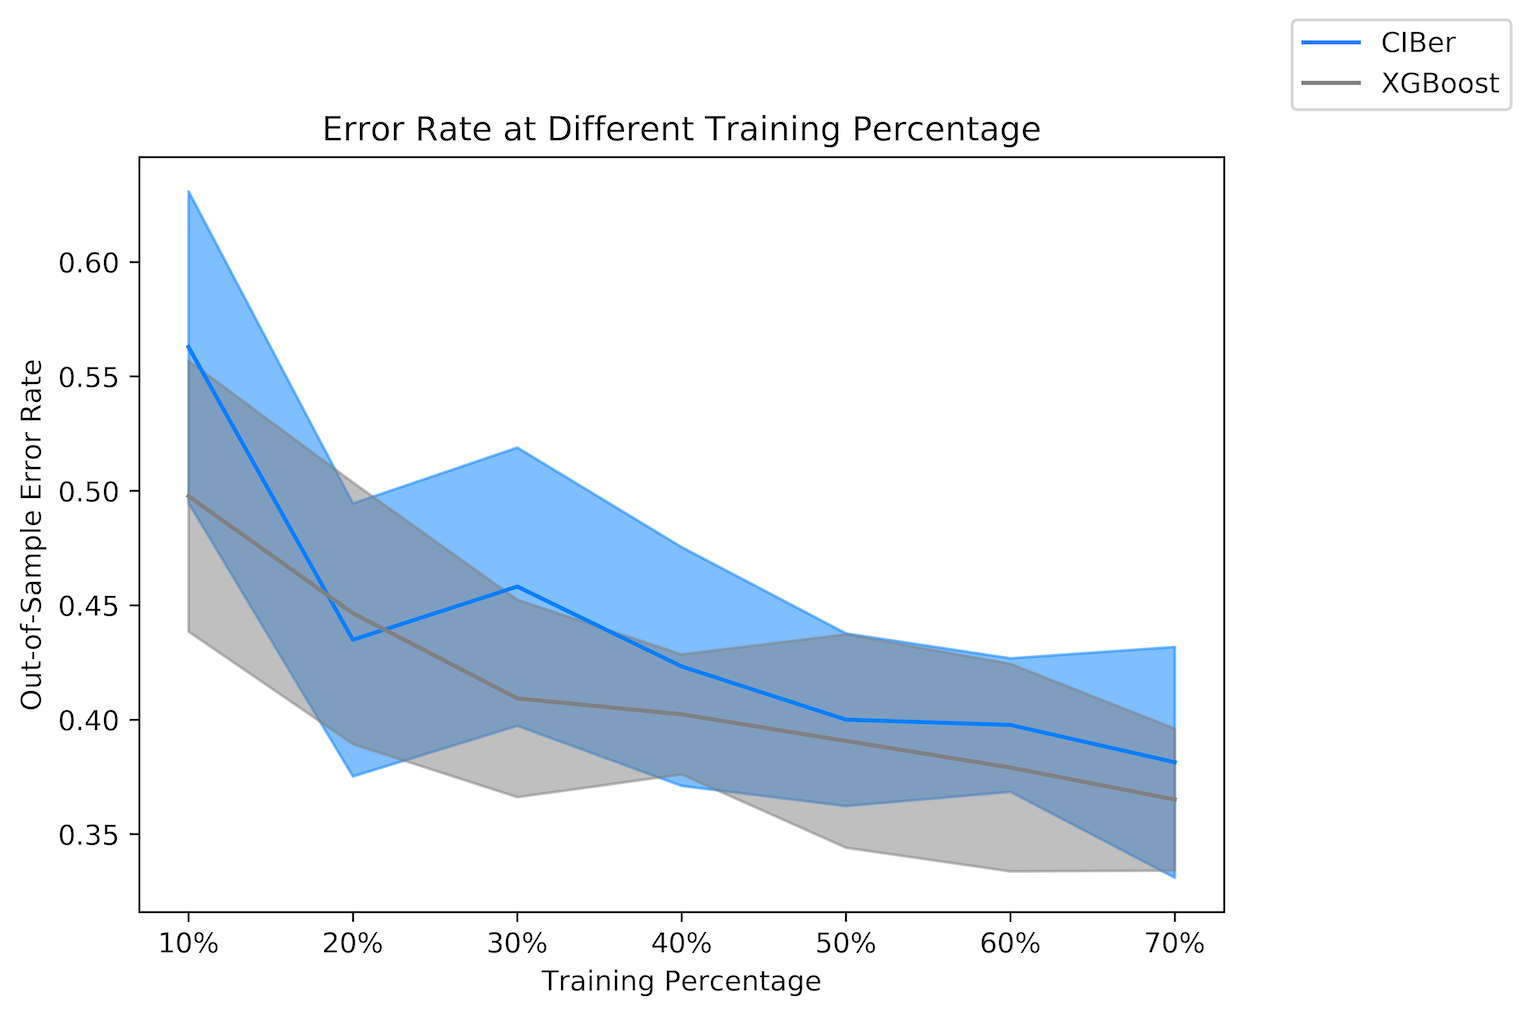
\includegraphics[width=0.85\linewidth]{Figures/Empirical/err_change_glass_xgb.png}
  \end{minipage}
  \begin{minipage}[b]{0.5\linewidth}
    \centering
    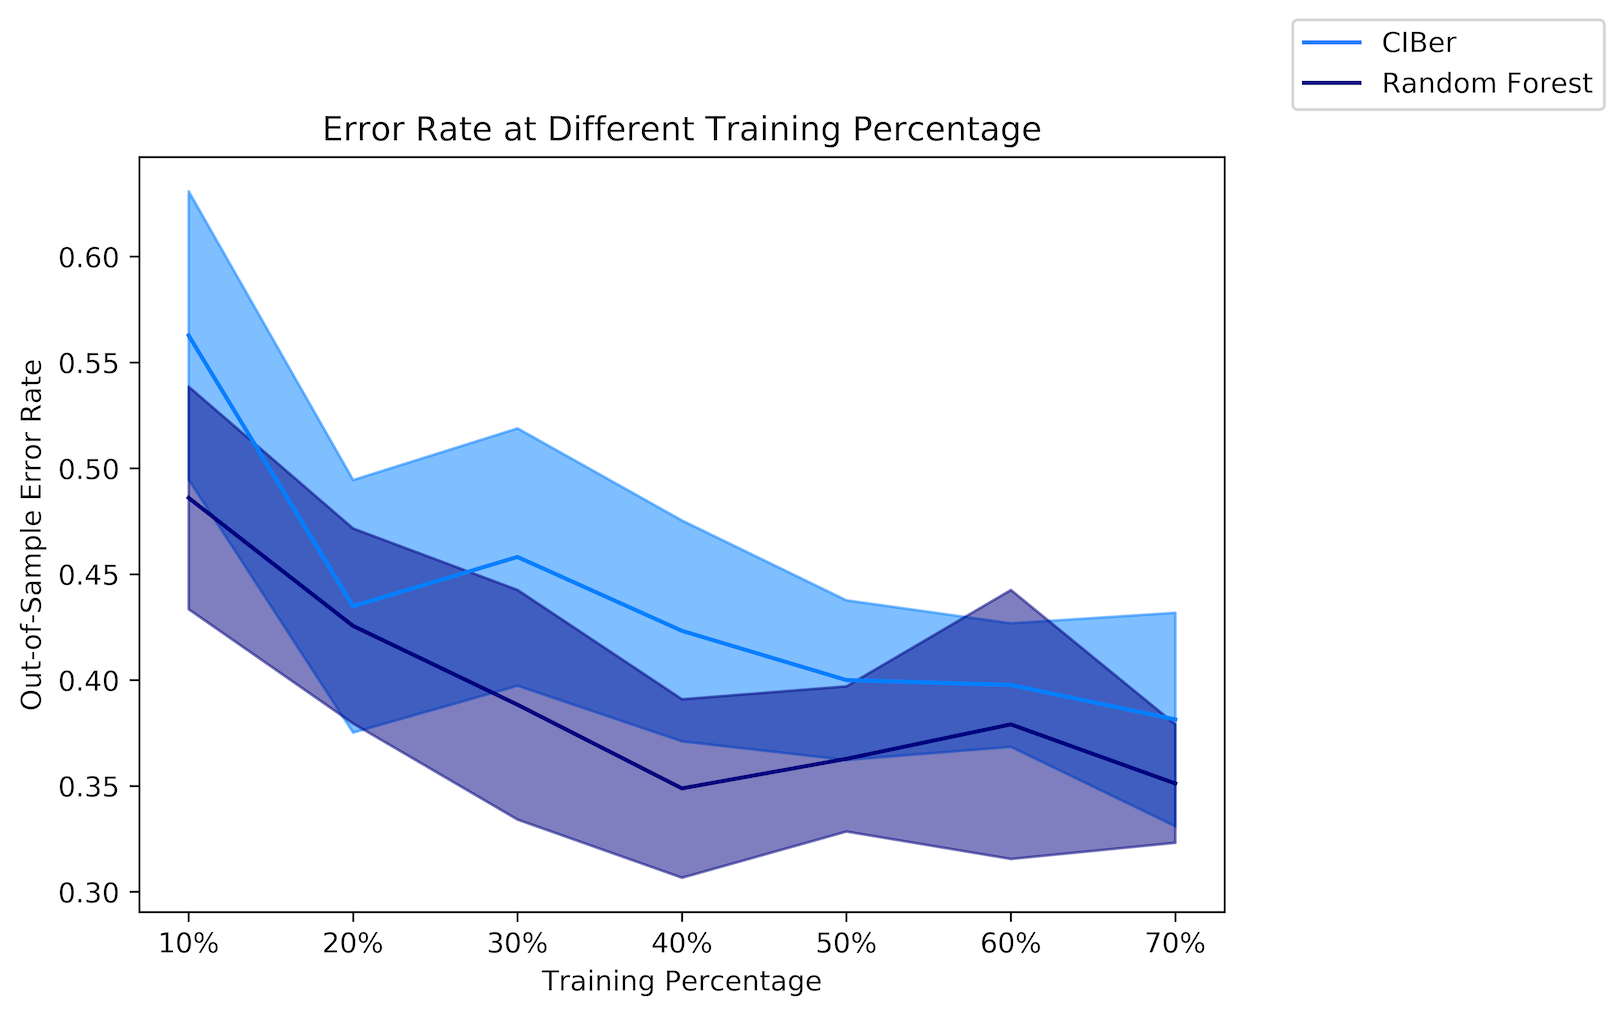
\includegraphics[width=0.9\linewidth]{Figures/Empirical/err_change_glass_rf.png}
  \end{minipage} 
  \caption{Change of Error Rate, Glass Identification Data-set} 
  \label{Fig_glass}
\end{figure}

As indicated by the larger band-width compared to the previous two data-sets, the performance variance of all models on this data-set becomes larger. This might be due to the small number of instances and a comparatively larger number of classes, which makes the estimation of conditional marginal probability imprecise. In the upper right sub-plot, the error rate of CIBer becomes smaller than the other models when the training percentage is above $40\%$. When compared with XGboost and random forest, the stabilities are similar since the bandwidths do not differ in a large scale. Even though CIBer's error rates are a bit larger than the two state-of-the-art models, there is still much intersection in the bands. We ascribe such deficiency to the lack of ensemble learning in CIBer. 


\subsection{Case Study: Financial Distress Prediction}
Now that we have shown the experimental results on data-sets from $4$ different domains, we conduct a case study about the classification of financial distress based on tens of financial and non-financial indicators. There are a number of open data-sets for this sort of tasks on data science platforms like Kaggle, and some of them are in the style of panel data in which multiple records for the same company at different time points exist simultaneously. For the simplicity of analysis, we disregard the potential autoregressive effects and just treat it as a classification task with multivariate inputs. Unlike the previous experiments in which we observed the trend of accuracy score when gradually enlarging the training size, we shall delve deeper into the hidden order captured by CIBer in this section. Meanwhile, apart from accuracies, we shall also compare the precision, recall, and F1-score simultaneously. We tuned the hyper-parameters by conducting a grid-search in order to find the optimal combination of minimum correlation and correlation type. Finally, we set the minimum correlation as $0.92$ and the correlation type as \textit{Spearman's Rho}. The results are shown in table \ref{fina_result}. For the columns of \textit{Precision}, \textit{Recall}, and \textit{F1-score}, in each parenthesis, the first element is the result on class $0$ and the second element is the result on class $1$. 

\begin{table}
\centering
 \begin{tabular}{||c c c c c||}
 \hline
 Model & Precision & Recall & F1-score & Accuracy\\ [0.5ex] 
 \hline\hline
 CIBer & (0.98,0.33) & (0.96,0.46) & (0.97,0.39) & 0.95 \\ 
 \hline
 Na\"ive Bayes & (0.99,0.08) & (0.60,0.88) & (0.74,0.14) & 0.61 \\
 \hline
 XGBoost & (0.97,0.33) & (0.98,0.27) & (0.98,0.30) & 0.95 \\
 \hline
 Random Forest & (0.97,0.31) & (0.98,0.24) & (0.98,0.27) & 0.95 \\
 \hline
 Decision Tree & (0.97,0.19) & (0.95,0.29) & (0.96,0.23) & 0.93 \\
 \hline
 SVM & (0.98,0.25) & (0.95,0.44) & (0.96,0.32) & 0.93 \\
 \hline
 Logistic Regression & (0.99,0.19) & (0.88,0.73) & (0.93,0.30) & 0.88 \\ [1ex] 
 \hline
 \end{tabular}
\caption{Results for Financial Distress Data-set}
\label{fina_result}
\end{table}

It can be observed that the disparity of overall accuracies among CIBer, XGBoost, Random Forest, Decision Tree and SVM is not significant. However, CIBer achieves the highest F1-score on the minority class while the F1-score on the majority class is just a little bit lower than the highest. Thus, the results indicate the strong competitiveness for CIBer in bankruptcy prediction. Next, we investigate the clusters formed by CIBer.

The features are numbered from $0$ to $82$, and the clusters of different sizes are listed out in table \ref{fina_cluster}. In the second column, indices of features within the same cluster are put inside the same parenthesis. 

\begin{table}
\centering
 \begin{tabular}{||c | c||}
 \hline
 Cluster Size & Clusters\\ [0.5ex]
 \hline\hline
 5 & (2, 12, 13, 46, 48) \\
 \hline
 4 & (1, 7, 35, 45) \\
 \hline
 3 & (67, 74, 75) \\
 \hline
 2 &
 \begin{tabular}{c} 
 (0, 5),(8, 24),(9, 80),(14, 34) \\
 (15, 51),(16, 33),(17, 19),(22, 49) \\ 
 (28, 32),(41, 54),(57, 58) \\
 \end{tabular} \\
 \hline
 \end{tabular}
\caption{Clusters formed by CIBer}
\label{fina_cluster}
\end{table}

We first take a look at the pair-plots of the largest cluster. As shown in Figure \ref{cluster_size5}, apart from $X_{46}$, the remaining features all approximately follow pair-wise comonotonicity. Thanks to \textit{Spearman's Rho}'s capability to capture both the linear and non-linear dependence, unlike \textit{Pearson's r} which only captures linear relationship, feature pairs like $(X_2, X_{12})$, $(X_2, X_{13})$, $(X_{12}, X_{13})$ whose pair-plots even indicate strict comonotonicity have been successfully recognized. This sufficiently increases the benefits brought by the comonotonicity paradigm. 

\begin{figure}
    \centering
    \includegraphics[scale = 0.4]{Figures/Empirical/cluster size5.png}
    \caption{Pair-plot of cluster with size 5}
    \label{cluster_size5}
\end{figure}

Apart from the largest cluster, the cluster with size $3$ also shows the advantage of comonotonity obviously. As shown in Figure \ref{cluster_size3}, the plot of any feature pair from the cluster $(X_{67}, X_{74}, X_{75})$ demonstrates a strictly positive dependence between each other. Moreover, we find from the plots on the diagonal entries that there is a lot of coincidence in the empirical class-wise distributions, which is much similar to the case in the simulation study. In this circumstance, if we, on the contrary, assume they are mutually independent, then the conditional joint probability of the $3$ features for the two classes must be too close to make a distinction, and thus contributes nothing to classification. In this way, it is approximately equivalent to simply discarding these three features, which reduces the information ``learned'' by the classifier, and deteriorates the prediction capability. Such things also happen for some clusters of size $2$. Figure \ref{cluster_size2} has shown two comonotonic feature pairs, and we can see that in each pair-plot, there is a large area of intersection under the two curves of empirical distribution. Moreover, as we have stated in the intuitive example \ref{intuitive_example}, when considering only two features, Na\"ive Bayes loses much power of judgement if the data satisfies the following conditions:
\begin{itemize}
    \item The two features are comonotonic.
    \item For both features, the differences in conditional marginal distribution on each class are small.
\end{itemize}
Hence, Figure \ref{cluster_size2} also indicates that using comonotonicity is better than Na\"ive Bayes at least for $(X_0, X_5)$ and $(X_{28}, X_{32})$. We confirm this claim by adjusting the training set and testing set, and then comparing the power of judgement between CIBer and Na\"ive Bayes. In more details, we conduct $2$ sets of experiments. In the first one, we only keep $(X_0, X_5)$, while in the second one we only keep $(X_{28}, X_{32})$. The feature selection is conducted after data preprocessing, including train-test-split, scaling, outlier removal, and generating synthetic data for the training set. In order to make our confirmation more solid, for both models, we discretize each feature into $20$ bins with equal length. The results are shown in table \ref{selected_features}. Since this is only to verify our claim that CIBer works better than Na\"ive Bayes when the data satisfies the two conditions above, we do not need to care about the absolute predictive power, but just need to compare the relative predictive power. After all, we only used two features for prediction, the noise of empirical data makes the gap between simulation and empirical experiments unable to be filled. From the table, we observe that in both experiments, CIBer has a better predictability than Na\"ive Bayes. Hence, our claim has been confirmed not only by simulation but also by empirical experiments.

\begin{figure}
    \centering
    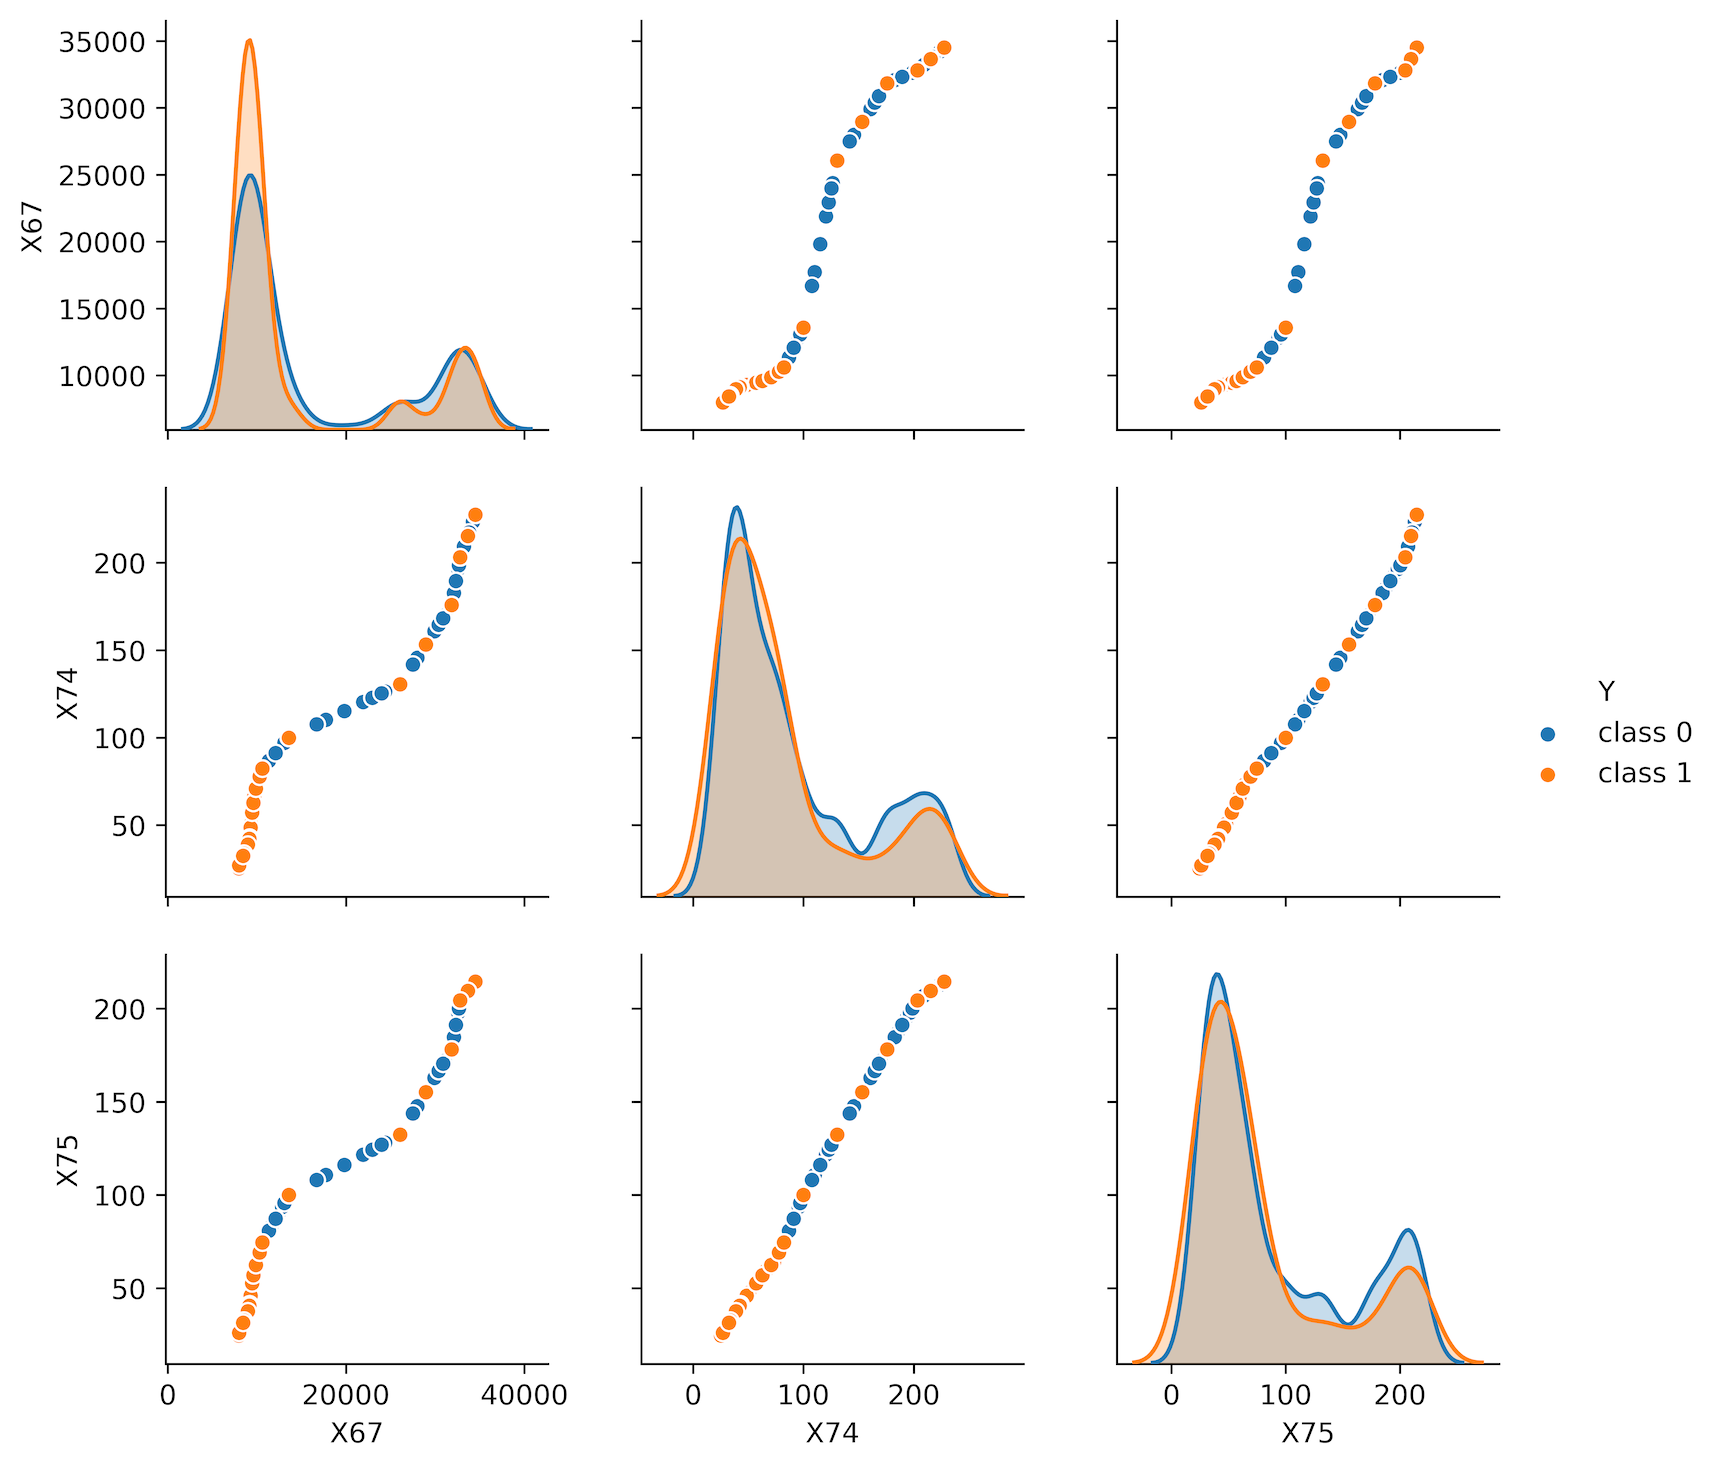
\includegraphics[scale = 0.4]{Figures/Empirical/cluster size3.png}
    \caption{Pair-plot of cluster with size 3}
    \label{cluster_size3}
\end{figure}

\begin{figure}[h]
\begin{tabular}{ll}
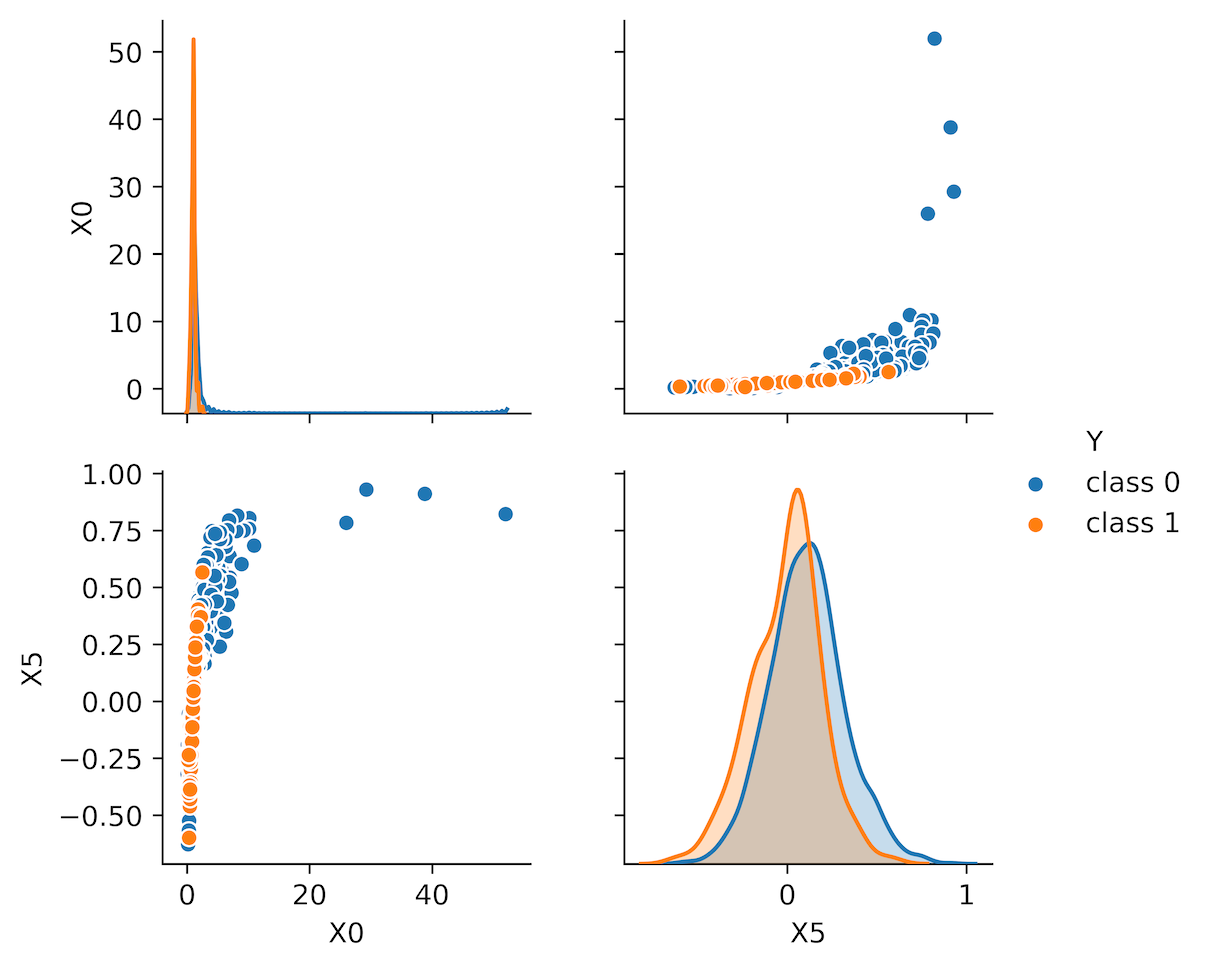
\includegraphics[scale=0.5]{Figures/Empirical/cluster size1_1.png}
&
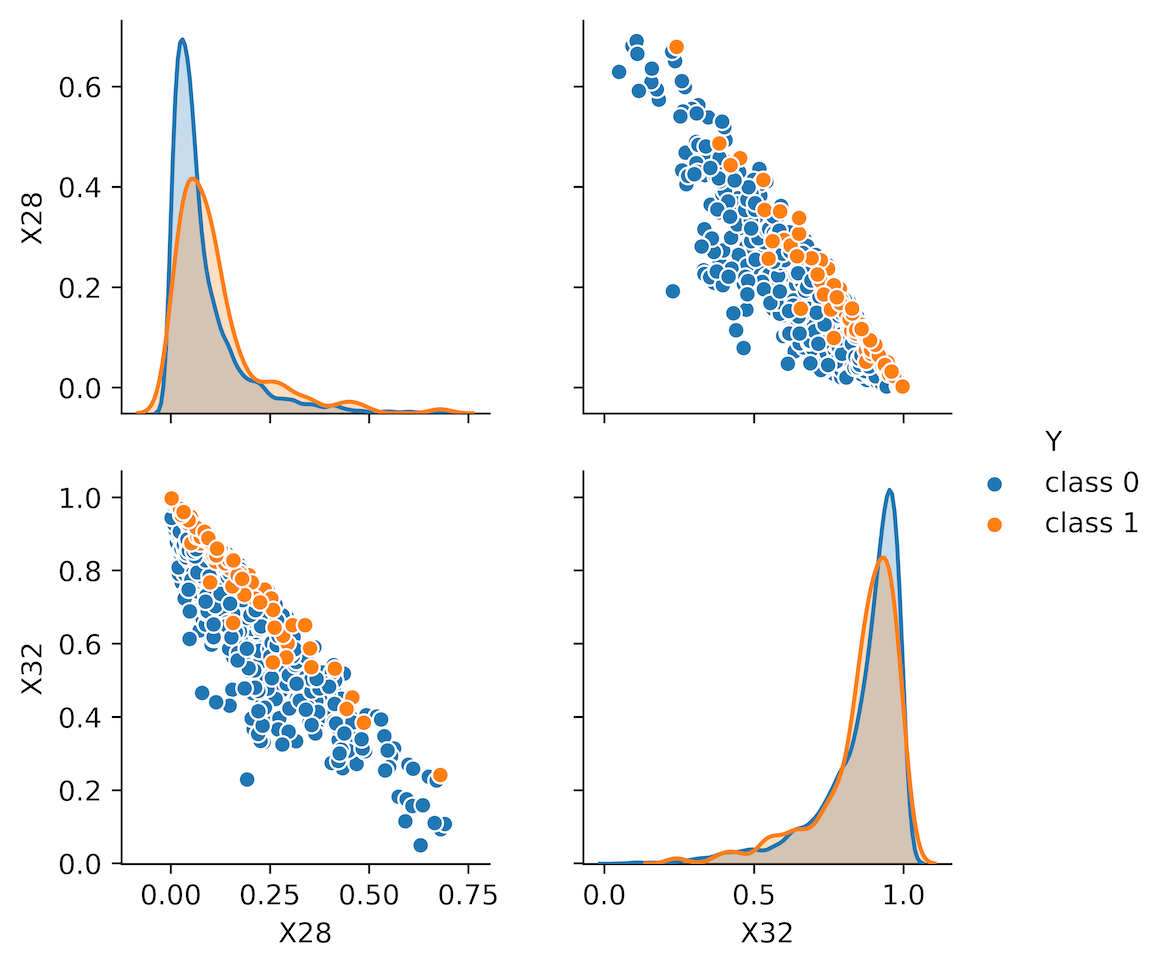
\includegraphics[scale=0.5]{Figures/Empirical/cluster size1_2.png}
\end{tabular}
\caption{Pair-plots of clusters with size 2} 
\label{cluster_size2}
\end{figure}

\begin{table}
\centering
 \begin{tabular}{||c c c c c c||}
 \hline
 Model & Selected Features & Precision & Recall & F1-score & Accuracy\\ [0.5ex] 
 \hline\hline
 CIBer & ($X_{0}$,$X_{5}$) & (0.98,0.07) & (0.60,0.76) & (0.74,0.12) & 0.60 \\ 
 \hline
 Na\"ive Bayes & ($X_{0}$,$X_{5}$) & (0.99,0.07) & (0.57,0.78) & (0.72,0.12) & 0.58 \\
 \hline
 CIBer & ($X_{28}$,$X_{32}$) & (0.95,0.03) & (0.43,0.44) & (0.59,0.05) & 0.43 \\ 
 \hline
 Na\"ive Bayes & ($X_{28}$,$X_{32}$) & (0.94,0.03) & (0.34,0.44) & (0.50,0.05) & 0.35 \\
 \hline
 \end{tabular}
\caption{Prediction only by selected features}
\label{selected_features}
\end{table}

\section{Conclusion}\label{conclusion}
Although Na\"ive Bayes has demonstrated high accuracy and efficiency in many scenarios, there were still many previous works aiming to tackle the problem brought by the violation of conditional independence, and they have achieved different levels of performance enhancement. Unlike the popular ideologies to improve Na\"ive Bayes, which incorporate attribute weighting or constructing a new feature set or adding extra arcs to the Na\"ive Bayesian network, CIBer conducts a heuristic search to find an optimal partition for the features, and then uses the measurement under the comonotonic paradigm to estimate the conditional joint probability. Thus, to some extent, CIBer brings a brand new ideology for Bayesian classifiers. Our simulation results have shown the reasonability of CIBer in some specific data distributions. Moreover, the strong stability and competitive performances compared to the state-of-the-art models on empirical data-sets further demonstrated the potential of CIBer. 

In the future, much improvements and alternatives of CIBer can be investigated. The current version of CIBer only considers continuous features. In the future, we hope to discover an appropriate way to deal with categorical features so that CIBer can be used in much more scenarios. At that time, more data-sets can be used to verify its power. Meanwhile, as inspired by Random Forest, we can apply ensemble learning technique in which multiple CIBer objects are fitted by the training data and the prediction is determined by voting. Additionally, there might exist more efficient heuristic search methods to find the optimal partition for the features. Last but not least, if we regard the comonotonic features as a meta-feature, then this might also be integrated into the Bayesian networks.

\bibliographystyle{plain}
\bibliography{ref}

\end{document}